% Acta Mechanica submission source: Springer Nature mathematics/physics numeric style.
% Single-column working version; journal guidelines recommend iicol for submission.
\documentclass[pdflatex,sn-mathphys-num]{sn-jnl}
\usepackage{graphicx}
\usepackage{amsmath,amssymb,amsfonts,bm,amsthm}
\usepackage{mathrsfs,booktabs,multirow,array,tabularx,dcolumn}
\graphicspath{{figures/}}
\emergencystretch=2em
\raggedbottom
\begin{document}
\title[Thermal expansion and voltage polarity]{Influence of Anisotropic Thermal Expansion on Voltage Polarity in a Thermopiezoelectric Microcantilever}
\author[1]{\fnm{Anjali} \sur{Patel}}
\author[2]{\fnm{Sandeep} \sur{Kumar}}
\author[3]{\fnm{Mohd} \sur{Vasiulla}}
\author[4]{\fnm{Arun Kumar} \sur{Yadav}}
\author*[5]{\fnm{Vipin} \sur{Gupta}}\email{vipin@gurugramuniversity.ac.in}
\affil[1]{\orgdiv{Department of Computer Science and Engineering, Amrita School of Artificial Intelligence Bengaluru}, \orgname{Amrita Vishwa Vidyapeetham}, \orgaddress{\city{Bengaluru}, \country{India}}}
\affil[2]{\orgdiv{Department of Mathematics}, \orgname{CDLU}, \orgaddress{\city{Sirsa}, \postcode{125055}, \state{Haryana}, \country{India}}}
\affil[3]{\orgdiv{Department of Mathematics, School of Computer Science \& Artificial Intelligence}, \orgname{SR University}, \orgaddress{\city{Warangal}, \postcode{506371}, \state{Telangana}, \country{India}}}
\affil[4]{\orgdiv{School of Basic and Applied Sciences}, \orgname{K.R. Mangalam University}, \orgaddress{\city{Gurugram}, \country{India}}}
\affil*[5]{\orgdiv{Department of Mathematics}, \orgname{Gurugram University}, \orgaddress{\city{Gurugram}, \postcode{122505}, \country{India}}}
\abstract{This paper studies the influence of anisotropic thermal expansion on the coupled piezoelectric--pyroelectric response of a tetragonal barium titanate microcantilever subjected to a steady through-thickness temperature difference. A plane-strain finite-element model is formulated from a single electric enthalpy, retaining the full three-dimensional thermal-stress contraction and the fixed-strain pyroelectric coefficient. The analysis separates the direct pyroelectric and thermally induced piezoelectric mechanisms to examine their contributions to the open-circuit voltage. The results show that neglecting constrained transverse thermal expansion substantially underestimates the thermal loading and can predict the wrong voltage polarity. Retaining this contribution changes the piezoelectric-thermal voltage from approximately $-0.22$~V to $+0.19$~V. The coupled response also demonstrates that piezoelectric feedback modifies the direct pyroelectric contribution, so the separately computed limiting cases cannot simply be added. The numerical solution is verified using an exact one-dimensional pyroelectric limit, mesh convergence and algebraic and variational consistency checks. A sensitivity analysis examines the dependence of voltage polarity on the thermal-expansion coefficients. The findings highlight the role of mechanical compatibility and constitutive consistency in predicting the electrical response of anisotropic thermopiezoelectric microstructures.}
\keywords{Anisotropic thermoelasticity, Plane strain, Thermopiezoelectricity, Voltage polarity, Barium titanate, Finite element method}
\maketitle
\section*{Nomenclature}
\begin{tabularx}{\linewidth}{@{}lX@{}}
\toprule
\textbf{Symbol} & \textbf{Description}\\
\midrule
$\bm u$ & Displacement vector\\
$\phi$ & Electric potential\\
$\varepsilon_{ij}$ & Strain tensor\\
$\gamma_{xz}$ & Engineering shear strain\\
$\sigma_{ij}$ & Stress tensor\\
$D_i$ & Electric displacement\\
$E_i$ & Electric field\\
$\theta$ & Temperature increment\\
$C_{ijkl}$ & Elastic stiffness tensor\\
$e_{kij}$ & Piezoelectric tensor\\
$\kappa_{ij}$ & Permittivity tensor\\
$p_i$ & Primary pyroelectric coefficient\\
$\alpha_{ij}$ & Thermal-expansion tensor\\
$\beta_{ij}$ & Thermal-stress coefficient\\
$\mu_{ijkl}$ & Flexoelectric tensor\\
$\ell$ & Internal material length\\
$L$ & Cantilever span\\
$h$ & Cantilever thickness\\
$V_{\mathrm{oc}}$ & Open-circuit voltage\\
\bottomrule
\end{tabularx}

\section{Introduction}
%======================================================================

Pyroelectric materials convert a change in temperature into an electrical signal
through the temperature dependence of their spontaneous polarization. This property is
used in infrared detectors, thermal imaging and devices that harvest energy from
ambient or waste-heat temperature fluctuations ~\cite{Lang2005Pyro,Whatmore1986,Lubomirsky2012}.
A microcantilever is mechanically compliant, so a small temperature difference
across its thickness can produce a measurable bending response. Cantilevers of this
type are also widely used as test structures for piezoelectric energy harvesting. Pyroelectric crystals lack a centre of symmetry and can therefore also exhibit
piezoelectricity. A non-uniform temperature field in a pyroelectric device consequently
acts in two ways: directly, through the pyroelectric coefficient, and indirectly,
through the thermal strain it produces, which the piezoelectric effect converts into
charge. Separating these two
contributions, and finding how a given device geometry combines them, requires a fully
coupled thermo-electro-mechanical boundary-value problem. The quantity computed here is
the open-circuit voltage, the potential difference between the two electrodes when no
net charge flows. It does not depend on an external load and is the quantity that a
static voltmeter measures most directly.

In a common treatment the two contributions are estimated separately. The pyroelectric
voltage is obtained from a one-dimensional electrical argument, and the piezoelectric
part, when it is considered, from a simple thermal-stress estimate that does not follow
the full anisotropy of the thermal-expansion tensor. Section~\ref{sec:results} shows
that, for the clamped cantilever studied here, this simplification changes not only the
size of the piezoelectric-thermal voltage but also its sign. Coupled formulations in
which temperature enters as an independent field together with strain and electric
field, known as thermopiezoelectricity, were developed by Mindlin and by Nowacki
~\cite{Mindlin1972,Nowacki1975}. These formulations provide the basis for device models
in which a prescribed temperature field is the load, and they have since been used to
study coupled thermo-piezoelectric waves and vibrations in orthotropic
hygro-thermo-piezoelastic media ~\cite{Gupta2024JNMP}, in piezo-thermo-electric
semiconductors ~\cite{Gupta2024WRCM,Gupta2025HFF} and in porous piezo-thermoelastic
solids ~\cite{Das2026KG}.

Barium titanate (BaTiO$_3$) is a suitable material for such a study. Its
room-temperature tetragonal phase has a complete, independently measured set of
elastic, piezoelectric and dielectric constants ~\cite{Zgonik1994,Berlincourt1958}. Its
ferroelectric phase transitions were established in classical single-crystal studies
~\cite{Merz1949,KayVousden1949} and explained by Devonshire's phenomenological theory
~\cite{Devonshire1949,Devonshire1951}. The crystal is also thermally anisotropic: on
heating, the $a$ axis of the tetragonal cell expands while the $c$ axis contracts, as
shown by variable-temperature diffraction ~\cite{Nakatani2016} and by thermal-expansion
measurements on related barium titanate-based ceramics ~\cite{Han2015,He2015Thermal}.
The anisotropic expansion enters the mechanical problem through standard
thermoelasticity ~\cite{BoleyWeiner1997,Nowacki1975}, but its plane-strain form for a
tetragonal crystal requires retaining the constrained transverse thermal expansion.
If the thermal expansion in the constrained out-of-plane direction is dropped before
the three-dimensional thermal stress is formed, the thermal load that drives both the
mechanical and the electrical response is misrepresented (Section~\ref{sec:planestrain}).
The effect is not represented in a strictly one-dimensional reduction; in the present
tetragonal plane-strain problem, however, the constrained out-of-plane expansion
contributes through the coupling terms involving the off-diagonal elastic constants.

A second point concerns the pyroelectric coefficient itself. Pyroelectricity consists
of a primary part, defined at fixed strain, and a secondary part caused by thermal
expansion acting through the piezoelectric effect in a mechanically free sample. Their
sum is the total (free) coefficient usually reported from bulk measurements
~\cite{Lang2005Pyro,Tagantsev1991,Lubomirsky2012}. A constitutive law written in terms
of strain, electric field and temperature requires the primary coefficient, because the
secondary part is produced by the piezoelectric term acting on the computed strain
field; using the total coefficient would count this part twice. The total coefficient
is commonly tabulated for ceramics, whereas the primary coefficient requires a more
specialized measurement or calculation. A recent first-principles study of tetragonal
BaTiO$_3$ reports the primary, secondary and total coefficients from one consistent
calculation ~\cite{EklundKarttunen2023}, and it provides the primary coefficient used here.

Both the primary and the secondary effects assume a uniform change of temperature. A
non-uniform temperature field, and the non-uniform strain it produces, gives rise to
what is called the tertiary pyroelectric effect ~\cite{Lang2005Pyro}. One of the cases
studied below (Case~E), in which a through-thickness temperature gradient acts on the
crystal with only the piezoelectric coupling active, is a finite-element treatment of
this tertiary mechanism for a specific geometry. Thermal-stress enhancement of the
pyroelectric response has recently been demonstrated experimentally in a polymer/mica
bimorph ~\cite{Su2026ThermalStressPyro}, where the stress comes from the
thermal-expansion mismatch between two layers. The present work considers a different
situation, a single tetragonal crystal under a through-thickness gradient, with
particular attention to the polarity of the voltage.

Flexoelectricity couples polarization to strain gradients and can become important
at small structural length scales. It is therefore
relevant to the strongly curved bending fields of microcantilevers
~\cite{Tagantsev1986,Cross2006,Zubko2013}, including barium titanate ~\cite{MaCross2006}
and cantilever geometries similar to the present one
~\cite{Huang2007,Mao2016,Abdollahi2014}. A consistent flexoelectric term requires an
internal material length scale, which rests on the strain-gradient theories of Toupin
and Mindlin ~\cite{Toupin1962,Mindlin1964,MindlinEshel1968}. The formulation below
contains this term for generality, while the voltages reported here are computed
without it (Section~\ref{sec:flexo}). Size-dependent flexoelectric and flexomagnetic
effects have also been shown to change the dispersion and attenuation of shear waves in
layered structures with imperfect or irregular interfaces
~\cite{Meghana2025,Gupta2026AMM}.

Once realistic boundary conditions are imposed, the coupled problem has no simple
closed-form solution. The plane-strain constraint and the through-thickness temperature
gradient produce a strain field that varies in space in a way that a one-dimensional or
lumped model cannot represent, and this non-uniform strain controls the sign of the
piezoelectric-thermal voltage. Finite-element formulations have been developed for such
coupled-field problems ~\cite{ZienkiewiczTaylor2005,Hughes2000,Belytschko2000,Bathe1996}.
Its piezoelectric form goes back to Allik and Hughes ~\cite{AllikHughes1970}, and it was
followed by two- and three-dimensional device models ~\cite{Lerch1990,Tzou1993} and
reviewed by Benjeddou ~\cite{Benjeddou2000a}. Studies of layered piezoelectric
composites have further shown how material gradation and interface conditions control
the coupled electromechanical response ~\cite{Gupta2025CS}. Thermopiezoelectric finite-element beam
models have been used for the vibration and active control of piezolaminated beams
under thermal disturbance ~\cite{Sanbi2014ThermoPyroBeam}; the present work addresses a
different question, the static open-circuit voltage of a single crystal and its
polarity. The higher-order extension of the formulation requires $C^1$
continuous mechanical interpolation. We use the classical
Bogner--Fox--Schmit (BFS) rectangular element ~\cite{Bogner1965}, which supplies this continuity without the extra
interface unknowns of mixed or penalty-based $C^0$ formulations. The reported
results have the flexoelectric contribution switched off; the BFS element is
therefore an implementation choice for these classical coupled-field calculations,
not a necessary consequence of their governing equations.

The mechanics question addressed here is how constrained anisotropic thermal
expansion changes the magnitude and sign of an electrical response. The
three-dimensional contraction defining the thermal-stress tensor and the distinction
between fixed-strain and free pyroelectric coefficients are established constitutive
requirements; they are not proposed as new constitutive laws. The contribution of
this study is to quantify their consequences for voltage polarity in a specified
plane-strain boundary-value problem. We (i) retain the constrained transverse
thermal expansion when constructing the thermal load; (ii) use a fixed-strain
pyroelectric coefficient to avoid double counting strain-mediated polarization;
(iii) propagate uncertainty in thermal-expansion coefficients obtained from
single-crystal diffraction data; (iv) verify the discrete solution using an exact
pyroelectric limit and algebraic identities; and (v) separate the electrical
mechanisms through mesh-converged coupled and uncoupled calculations. These
comparisons show why a free-sample estimate need not predict the sign of a
constraint-dependent thermopiezoelectric response.


%======================================================================
\section{Mathematical Formulation}
\label{sec:theory}
%======================================================================

\subsection{Physical assumptions and kinematics}

The body occupies the plane-strain domain $\Omega=\{(x,z):0\le x\le L,\ 0\le z\le h\}$
and consists of tetragonal $4mm$ BaTiO$_3$ poled along $z$. The displacement, electric
potential and temperature increment are $\bm u(x,z)=(u,0,w)$, $\phi(x,z)$ and
$\theta=T-T_0$, with $E_i=-\phi_{,i}$ and small-strain kinematics
$\varepsilon_{ij}=\tfrac12(u_{i,j}+u_{j,i})$. Plane strain imposes
$\varepsilon_{yy}=\varepsilon_{xy}=\varepsilon_{yz}=0$ and $\partial_y(\cdot)\equiv0$,
which leaves the active strains $\varepsilon_{xx}=u_{,x}$, $\varepsilon_{zz}=w_{,z}$
and $\gamma_{xz}=u_{,z}+w_{,x}$. In Voigt notation ~\cite{Nye1985,IEEE176} the active
strain vector is $\bm\varepsilon=[\varepsilon_{xx},\varepsilon_{zz},\gamma_{xz}]^\top$,
where the shear component is the engineering strain $\gamma_{xz}=2\varepsilon_{xz}$.
The factor of two appears once, in the strain vector, and the reduced stiffness and
coupling matrices are defined so that the products $C\bm\varepsilon$ and
$e\bm\varepsilon$ give the corresponding tensor contractions. With the index map
$11\to1$, $33\to2$, $13\to3$, and after deleting the rows and columns of the tetragonal
tensors that vanish under plane strain, the active stiffness, piezoelectric and
permittivity blocks used in \eqref{eq:elementmats} are
\begin{equation}
C=\begin{bmatrix}C_{11}&C_{13}&0\\C_{13}&C_{33}&0\\0&0&C_{44}\end{bmatrix},
\qquad
e=\begin{bmatrix}0&0&e_{15}\\e_{31}&e_{33}&0\end{bmatrix},
\qquad
\kappa=\begin{bmatrix}\kappa_{11}&0\\0&\kappa_{33}\end{bmatrix},
\label{eq:voigtblocks}
\end{equation}
taken from the full $6\times6$ and $3\times6$ tensors reported by Zgonik et al.
~\cite{Zgonik1994}.

\subsection{Constitutive relations}

The constitutive relations follow from a single electric enthalpy density per unit
volume,
\begin{equation}
H(\varepsilon,E,\theta)=\tfrac12 C_{ijkl}\varepsilon_{ij}\varepsilon_{kl}
-e_{kij}\varepsilon_{ij}E_k-\tfrac12\kappa_{ij}E_iE_j-\beta_{ij}\varepsilon_{ij}\theta
-p_iE_i\theta,
\label{eq:H}
\end{equation}
where $\beta_{ij}:=C_{ijkl}\alpha_{kl}$ is the thermal-stress coefficient and
$\alpha_{ij}$ the linear thermal-expansion tensor. The independent variables are the
total strain $\varepsilon$, the electric field $E$ and the temperature increment
$\theta$, which is the electric-enthalpy form used in piezoelectricity
~\cite{Tiersten1969b,Yang2005b}. Differentiation gives
\begin{equation}
\sigma_{ij}=\frac{\partial H}{\partial\varepsilon_{ij}}
=C_{ijkl}(\varepsilon_{kl}-\alpha_{kl}\theta)-e_{kij}E_k,
\qquad
D_i=-\frac{\partial H}{\partial E_i}
=e_{ikl}\varepsilon_{kl}+\kappa_{ij}E_j+p_i\theta,
\label{eq:constitutive}
\end{equation}
The thermal term appears as an eigenstrain in the stress, so that the material responds
to the elastic part of the total strain. The minus sign in
$D_i=-\partial H/\partial E_i$ gives positive contributions from the three electric
terms in $D_i$. Because $\varepsilon$ is the independent mechanical variable in
\eqref{eq:H}, the coefficient $p_i$ in \eqref{eq:constitutive} is the fixed-strain
(primary) pyroelectric coefficient. The free (total) coefficient belongs to a different
potential obtained from $H$ by the corresponding Legendre transform with respect to
strain. Using the free coefficient in \eqref{eq:constitutive} would include the
strain-mediated contribution in addition to the contribution already generated by
$e_{ikl}\varepsilon_{kl}$. Section~\ref{sec:materials} returns to this distinction when
the material data are selected.

\subsection{Plane-strain reduction of the thermal-stress vector}
\label{sec:planestrain}

For tetragonal $4mm$ symmetry, $\alpha_{xx}=\alpha_{yy}=\alpha_1$ and
$\alpha_{zz}=\alpha_3$, and the full three-dimensional normal-stress block is
\begin{equation}
\begin{Bmatrix}\sigma_{xx}\\\sigma_{yy}\\\sigma_{zz}\end{Bmatrix}
=
\begin{bmatrix}
C_{11}&C_{12}&C_{13}\\
C_{12}&C_{11}&C_{13}\\
C_{13}&C_{13}&C_{33}
\end{bmatrix}
\begin{Bmatrix}\varepsilon_{xx}\\\varepsilon_{yy}\\\varepsilon_{zz}\end{Bmatrix}
-
\begin{Bmatrix}\beta_{xx}\\\beta_{yy}\\\beta_{zz}\end{Bmatrix}\theta,
\qquad
\begin{Bmatrix}\beta_{xx}\\\beta_{yy}\\\beta_{zz}\end{Bmatrix}
=
\begin{bmatrix}
C_{11}&C_{12}&C_{13}\\
C_{12}&C_{11}&C_{13}\\
C_{13}&C_{13}&C_{33}
\end{bmatrix}
\begin{Bmatrix}\alpha_1\\\alpha_1\\\alpha_3\end{Bmatrix}.
\label{eq:beta3d}
\end{equation}
Plane strain sets the \emph{total} strain $\varepsilon_{yy}$ to zero, not the thermal
eigenstrain $\alpha_1\theta$. The thermal expansion in the $y$ direction therefore
still contributes to $\sigma_{xx}$ and $\sigma_{zz}$ through $C_{12}$ and $C_{13}$ in
\eqref{eq:beta3d}. The thermal-stress vector used in the plane-strain problem is
\begin{equation}
\beta_{\mathrm{PS}}
=
\big[(C_{11}{+}C_{12})\alpha_1+C_{13}\alpha_3,\ \
2C_{13}\alpha_1+C_{33}\alpha_3,\ \
0\big]^{\!\top},
\label{eq:betaPS}
\end{equation}
obtained by taking the $xx$ and $zz$ components of \eqref{eq:beta3d} after the full
three-dimensional contraction has been formed. A simplified reduction applies the
two-component plane-strain stiffness directly to $[\alpha_1,\alpha_3,0]^\top$ and
therefore misses the term $C_{12}\alpha_1$ in $\beta_{xx}$ and one of the two terms
$C_{13}\alpha_1$ in $\beta_{zz}$. With the material data of Section~\ref{sec:materials},
\eqref{eq:betaPS} gives
$\beta_{\mathrm{PS}}=[6.7167,\,4.1903,\,0]^\top\times10^{6}\,\text{Pa\,K}^{-1}$,
whereas the simplified reduction gives
$[4.3623,\,1.7705,\,0]^\top\times10^{6}\,\text{Pa\,K}^{-1}$
(Table~\ref{tab:beta}).

\begin{table}[t]
\centering
\caption{Plane-strain thermal-stress vector: simplified reduction versus the full
three-dimensional contraction, both evaluated at the same thermal-expansion
coefficients
($\alpha_1=+21.8\times10^{-6}\,\text{K}^{-1}$, $\alpha_3=-4.3\times10^{-6}\,\text{K}^{-1}$).}
\label{tab:beta}
\resizebox{\linewidth}{!}{%
\begin{tabular}{@{}lrrr@{}}
\toprule
Component & Simplified (Pa K$^{-1}$) & Full 3D contraction, Eq.~\eqref{eq:betaPS} (Pa K$^{-1}$) &
Underestimation \\
\midrule
$\beta_{xx}$ & $4.3623\times10^{6}$ & $6.7167\times10^{6}$ & $35.05\%$ \\
$\beta_{zz}$ & $1.7705\times10^{6}$ & $4.1903\times10^{6}$ & $57.75\%$ \\
\bottomrule
\end{tabular}%
}
\end{table}

Table~\ref{tab:beta} compares the two forms of the thermal-stress vector at the same
thermal-expansion coefficients. The simplified reduction retains about two thirds of
the axial component and less than half of the through-thickness component. The larger
difference in $\beta_{zz}$ results from the omitted contribution involving
$C_{13}\alpha_1$: the in-plane coefficient $\alpha_1$ is positive and relatively large,
whereas the retained term $C_{33}\alpha_3$ is negative because the $c$ axis contracts
on heating. Thus, the plane-strain constraint couples the in-plane thermal expansion
to both stress components through the off-diagonal elastic constants. Omitting these
contributions removes a substantial part of the thermal load. Both reductions give the
same sign of $\beta$; the difference in magnitude leads to the different voltage
response discussed in Section~\ref{sec:polarity}.

\subsection{Higher-order (flexoelectric) extension}
\label{sec:flexo}

The general formulation also contains an effective flexoelectric term,
$D_i^\mu=\mu_{ijkl}\eta_{jkl}$, with $\eta_{jkl}=\varepsilon_{jk,l}$ the strain
gradient, together with a strain-gradient elastic stiffness
$A=C_{44}\ell^2\mathbb{I}$ of Mindlin form~II, where $\ell$ is an internal material
length. Both are implemented reciprocally, as cross-derivatives of one enthalpy
augmented with the terms
$\tfrac12A_{jklmno}\eta_{jkl}\eta_{mno}-\mu_{kjkl}\eta_{jkl}E_k$, following the
strain-gradient theories of Toupin, Mindlin and Koiter
~\cite{Toupin1962,Mindlin1964,MindlinEshel1968} and their later engineering forms
~\cite{FleckHutchinson1997,Lam2003,AskesAifantis2011}, in line with recent flexoelectric
finite-element frameworks
~\cite{Mao2016,MaoPurohit2014,Abdollahi2014}. Effective flexoelectric tensors have
been obtained from first-principles and atomistic calculations for several perovskites
and other dielectrics
~\cite{MarangantiSharma2009,HongVanderbilt2011,Stengel2013}, and length scales have
been measured in flexoelectric barium titanate ceramics
~\cite{MaCross2006,Huang2007}. All voltages reported in this paper are computed with
$\mu_{ijkl}=0$ and $\ell=0$, so that they reflect the piezoelectric and pyroelectric
mechanisms only. The flexoelectric term is retained in the formulation so that the
same $C^1$-conforming discretization can be used when strain-gradient terms are
activated in a future extension.

\subsection{Boundary conditions}
\label{sec:bcs}

The cantilever is clamped at $x=0$. At every BFS node on this edge, all eight mechanical
degrees of freedom are set to zero,
$u=u_{,x}=u_{,z}=u_{,xz}=w=w_{,x}=w_{,z}=w_{,xz}=0$, as implemented in the BFS
discretization described in Section~\ref{sec:discretization}. The remaining edges are
traction-free. The bottom face ($z=0$) is a grounded electrode, $\phi=0$. The top face
($z=h$) is a floating electrode, a single equipotential surface with zero net charge
(open circuit); this condition is imposed as a discrete statement of total charge
balance over all electrical degrees of freedom on that face. A steady temperature field
that varies linearly through the thickness is prescribed,
$\theta(z)=\Delta T\,z/h$ with $\Delta T=10$~K and $T_0=300$~K, so that
$T(z)=300+10z/h$~K. All material coefficients are evaluated at $T_0$ and taken as
constant over this 10~K interval, which lies inside the 298--343~K range of the
thermal-expansion data (Section~\ref{sec:materials}) and matches the 300~K
pyroelectric coefficient (Table~\ref{tab:materials}).

\begin{figure}[t]
  \centering
  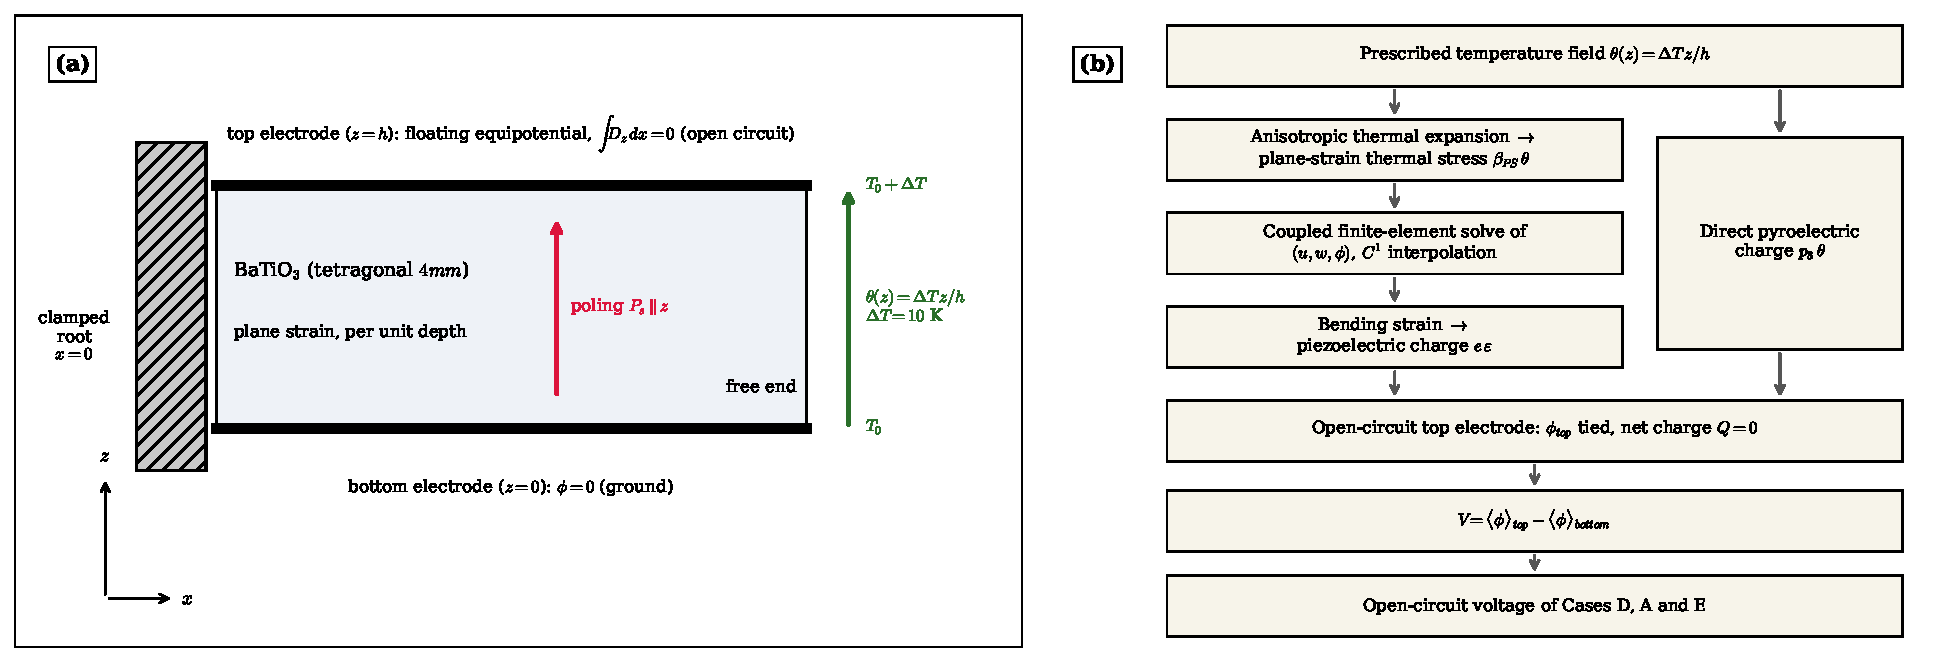
\includegraphics[width=\linewidth]{Fig1_model_schematic}
  \caption{Model configuration. (a) Specimen geometry ($L=10\,\mu$m, $h=1\,\mu$m;
  not to scale) with clamped root, poling direction, prescribed temperature gradient,
  grounded bottom electrode and open-circuit top electrode. (b) The two routes from
  the prescribed temperature to the open-circuit voltage: the mechanical route through
  thermal stress, deformation and piezoelectric charge, and the direct pyroelectric
  route.}
  \label{fig:fig01_model_schematic}
\end{figure}

Figure~\ref{fig:fig01_model_schematic} summarizes the model. Panel (a) shows the
specimen, 10~$\mu$m long and 1~$\mu$m thick, clamped at its left end and free at its
right end. The crystal is poled along $z$, the bottom electrode is grounded, the top
electrode floats, and the temperature rises linearly from the bottom face to the top
face. Panel (b) shows the two routes by which the prescribed temperature reaches the
voltage. In the mechanical route (left column), the anisotropic thermal expansion is
converted into thermal stress by the plane-strain constraint, the coupled problem is
solved, the cantilever bends, and the resulting strain produces charge through the
piezoelectric tensor. In the direct route (right column), the temperature changes the
polarization through the pyroelectric coefficient. Both routes end at the floating top
electrode, where the open-circuit condition fixes a single potential, and the voltage
reported in this paper is the difference between this potential and that of the grounded
bottom electrode. In the present crystal, the two routes produce voltages of opposite
sign. The way the thermal stress is formed from the thermal expansion therefore
determines how strongly the mechanical route offsets the direct pyroelectric
contribution.

%======================================================================
\section{Variational and Finite Element Formulation}
\label{sec:fem}
%======================================================================

\subsection{Weak formulation}

Stationarity of $\int_\Omega H\,dA$ with respect to the admissible variations
$\delta\bm u$ and $\delta\phi$, with
$\delta\varepsilon_{ij}=\tfrac12(\delta u_{i,j}+\delta u_{j,i})$ and
$\delta E_i=-\delta\phi_{,i}$, gives
\begin{equation}
\delta\!\int_\Omega H\,dA
=\int_\Omega\big(\sigma_{ij}\,\delta\varepsilon_{ij}
-D_i\,\delta E_i\big)\,dA=0,
\label{eq:stationarity}
\end{equation}
with \eqref{eq:constitutive}. Substituting
$\delta E_i=-\delta\phi_{,i}$ gives the coupled virtual-work statement
\begin{equation}
\int_\Omega\big(\delta\bm\varepsilon^{\!\top}\bm\sigma
+\nabla\delta\phi\cdot\bm D\big)\,dA=0
\qquad\text{for all admissible }\delta\bm u,\ \delta\phi.
\label{eq:weakform}
\end{equation}
With the interpolations $\bm u\approx N_uq_u$ and
$\phi\approx N_\phi q_\phi$ over each Bogner--Fox--Schmit element
(Section~\ref{sec:discretization}), the strain and electric field are
$\bm\varepsilon\approx B_\varepsilon q_u$ and
$\bm E\approx-B_\phi q_\phi$. Substituting these relations and the matrix form of
\eqref{eq:constitutive},
\[
\bm\sigma=C\bm\varepsilon-e^{\!\top}\bm E
-\bm\beta_{\mathrm{PS}}\theta,
\qquad
\bm D=e\bm\varepsilon+\kappa\bm E+\bm p\,\theta,
\]
into \eqref{eq:weakform} gives the monolithic block system
\begin{equation}
\begin{bmatrix}
K_{uu} & K_{u\phi}\\
K_{u\phi}^{\!\top} & -K_{\phi\phi}
\end{bmatrix}
\begin{Bmatrix}q_u\\q_\phi\end{Bmatrix}
=
\begin{Bmatrix}f_u\\f_\phi\end{Bmatrix},
\label{eq:global}
\end{equation}
with
\begin{align}
K_{uu}&=\int_\Omega B_\varepsilon^{\!\top}CB_\varepsilon\,dA, &
K_{u\phi}&=\int_\Omega B_\varepsilon^{\!\top}e^{\!\top}B_\phi\,dA, &
K_{\phi\phi}&=\int_\Omega B_\phi^{\!\top}\kappa B_\phi\,dA,\notag\\[2pt]
f_u&=\int_\Omega B_\varepsilon^{\!\top}\beta_{\mathrm{PS}}\,\theta\,dA, &
f_\phi&=-\int_\Omega B_\phi^{\!\top}\bm p\,\theta\,dA.& &
\label{eq:elementmats}
\end{align}
The negative sign in the electrical block follows from
$\bm E=-B_\phi q_\phi$. The resulting system is symmetric and indefinite, with a
positive-definite mechanical energy block and a negative-semidefinite electrical
block. The symmetry
$K_{\phi u}=K_{u\phi}^{\!\top}$ follows because the two coupling blocks arise from
mixed second derivatives of the same potential \eqref{eq:H}; the equality of these
mixed derivatives is also verified numerically in Section~\ref{sec:checks}.

\subsection{Finite-element interpolation}
\label{sec:discretization}

The mechanical fields are interpolated with the 16-function Bogner--Fox--Schmit
basis ~\cite{Bogner1965}. On the reference element
$\xi,\eta\in[-1,1]$, each mechanical component ($u$ or $w$) is represented by a
tensor-product cubic Hermite interpolation,
\begin{align}
u(\xi,\eta)=\sum_{a=1}^{4}\Big[&
H_0(-\xi_a\xi)H_0(-\eta_a\eta)\,u_a
-\xi_aH_1(-\xi_a\xi)H_0(-\eta_a\eta)\,u_{,\xi}^a\notag\\
&-\eta_aH_0(-\xi_a\xi)H_1(-\eta_a\eta)\,u_{,\eta}^a
+\xi_a\eta_aH_1(-\xi_a\xi)H_1(-\eta_a\eta)\,u_{,\xi\eta}^a\Big],
\label{eq:bfs-interp}
\end{align}
where the sum runs over the four corner nodes $a$, with
$\xi_a,\eta_a\in\{-1,+1\}$ denoting the reference coordinates of node $a$.
The functions $H_0$ and $H_1$ are the cubic Hermite functions satisfying
$H_0(1)=0$, $H_0(-1)=1$, $H_0'(\pm1)=0$,
$H_1(\pm1)=0$, $H_1'(1)=0$, and $H_1'(-1)=1$. The prefactors
$-\xi_a$, $-\eta_a$, and $\xi_a\eta_a$ on the derivative terms follow from the
reference-element construction and provide the required nodal value and derivative
properties. Explicitly,
\begin{equation}
H_0(s)=\tfrac14(2-3s+s^3),\qquad
H_1(s)=\tfrac14(1-s-s^2+s^3),
\label{eq:hermite}
\end{equation}
Each node therefore carries the field value, the two first derivatives, and the mixed
second derivative, giving four degrees of freedom per mechanical component and eight
mechanical degrees of freedom per node for the pair $(u,w)$. The BFS interpolation is
$C^1$ continuous, so the first derivatives of the displacement fields are continuous
across element boundaries. This property is required by the strain-gradient extension,
for which $\eta_{jkl}=\varepsilon_{jk,l}$ contains derivatives of the strain field.
The electric potential is interpolated with the standard four-node bilinear ($C^0$)
basis, while the prescribed temperature field is evaluated from the linear
through-thickness distribution specified in Section~\ref{sec:bcs}. The latter enters
the element equations through its values at the integration points.

\subsection{Strain-displacement and electrical operators}
\label{sec:Bops}

With the nodal mechanical unknowns ordered as
\[
q_u=(u_a,u_{,\xi}^a,u_{,\eta}^a,u_{,\xi\eta}^a,
w_a,w_{,\xi}^a,w_{,\eta}^a,w_{,\xi\eta}^a)_{a=1}^{4}\in\mathbb{R}^{32},
\]
the strain vector
$\bm\varepsilon=(\varepsilon_{xx},\varepsilon_{zz},\gamma_{xz})^\top
=B_\varepsilon q_u$ has $B_\varepsilon\in\mathbb{R}^{3\times32}$, constructed from
\eqref{eq:bfs-interp} and the Jacobian-scaled derivatives
$N_{,x}=J_x^{-1}N_{,\xi}$ and $N_{,z}=J_z^{-1}N_{,\eta}$:
\begin{align}
(B_\varepsilon)_{1,\,0:15}&=N_{,x}^\top,\quad
(B_\varepsilon)_{1,\,16:31}=\bm0;\notag\\
(B_\varepsilon)_{2,\,0:15}&=\bm0,\quad
(B_\varepsilon)_{2,\,16:31}=N_{,z}^\top;\notag\\
(B_\varepsilon)_{3,\,0:15}&=N_{,z}^\top,\quad
(B_\varepsilon)_{3,\,16:31}=N_{,x}^\top,
\label{eq:Beps}
\end{align}
Row~1 ($\varepsilon_{xx}=u_{,x}$) acts only on the $u$ degrees of freedom,
row~2 ($\varepsilon_{zz}=w_{,z}$) only on the $w$ degrees of freedom, and row~3
($\gamma_{xz}=u_{,z}+w_{,x}$) on both, following the kinematics of
Section~\ref{sec:theory}. The electric field is
$\bm E=-B_\phi q_\phi$, with
$B_\phi=(N_{\phi,x},N_{\phi,z})^\top\in\mathbb{R}^{2\times4}$ constructed from the
bilinear basis. On the finest mesh ($80\times40$), the elements are five times longer
than they are thick, so the $z$ derivatives are about five times larger than the
$x$ derivatives ($|N_{,z}|\sim8\times10^{7}\,\text{m}^{-1}$ against
$|N_{,x}|\sim1.6\times10^{7}\,\text{m}^{-1}$). This difference, together with the
different scales of the mechanical and electrical unknowns, motivates the scaling
described in Section~\ref{sec:assembly}.

\subsection{Element matrices and Gauss--Legendre quadrature}

Every element integral in \eqref{eq:elementmats} is evaluated on the reference square
$[-1,1]^2$ with a $4\times4$ Gauss--Legendre rule
~\cite{AbramowitzStegun1965,Gautschi2004},
\begin{equation}
\int_{\Omega_e}f\,dx\,dz
=\sum_{g=1}^{16}f(\xi_g,\eta_g)\,w_g\,J_xJ_z,
\label{eq:quad}
\end{equation}
with the one-dimensional abscissae and weights
\begin{equation}
\xi_g\in\{\pm0.86114,\ \pm0.33998\},\qquad
w_g\in\{0.34785,\ 0.65215\},
\label{eq:gaussweights}
\end{equation}
and two-dimensional weights formed as products of the one-dimensional weights.
For the cubic Hermite basis on a rectangular element, this quadrature rule integrates
the polynomial entries of $B_\varepsilon^{\!\top}CB_\varepsilon$ exactly, so the
corresponding element integrals have no quadrature error beyond round-off. The
element matrices and mechanical load vector are
\begin{align}
K_{uu}
&=\sum_{g=1}^{16}w_gJ_xJ_z\,
B_\varepsilon(\xi_g,\eta_g)^{\!\top}C
B_\varepsilon(\xi_g,\eta_g)
\in\mathbb{R}^{32\times32}, &
K_{u\phi}
&=\sum_{g=1}^{16}w_gJ_xJ_z\,
B_\varepsilon^{\!\top}e^{\!\top}B_\phi
\in\mathbb{R}^{32\times4},
\notag\\
K_{\phi\phi}
&=\sum_{g=1}^{16}w_gJ_xJ_z\,
B_\phi^{\!\top}\kappa B_\phi
\in\mathbb{R}^{4\times4}, &
f_u
&=\sum_{g=1}^{16}w_gJ_xJ_z\,
B_\varepsilon^{\!\top}\beta_{\mathrm{PS}}\,\theta_g
\in\mathbb{R}^{32},
\label{eq:elemsums}
\end{align}
with
$f_\phi=-\sum_g w_gJ_xJ_z\,B_\phi^{\!\top}\bm p\,\theta_g\in\mathbb{R}^4$
(Eq.~\eqref{eq:elementmats}). The electrical load $f_\phi$ contains no additional
thermal-strain term; the thermal contribution enters the electrical equation through
the prescribed pyroelectric term in \eqref{eq:constitutive}.

\subsection{Assembly and solution}
\label{sec:assembly}

The element blocks are assembled into the global sparse system through the usual
connectivity map ~\cite{Bathe1996}. The unknowns contain displacements, displacement
derivatives, and electric potentials, whose magnitudes differ by several orders.
The resulting raw system is therefore poorly conditioned. Before solution, the
reduced system is scaled by a diagonal congruence transformation,
\[
K\to S^{-1}KS^{-1},\qquad
q\to Sq,\qquad
f\to S^{-1}f,
\]
with $S$ a diagonal matrix. This transformation is an exact change of variables and
does not alter the physical solution. The scaled system is then solved with a direct
sparse solver.

%======================================================================
\section{Material Parameters}
\label{sec:materials}
%======================================================================

Table~\ref{tab:materials} lists the material parameters and their sources. The elastic,
piezoelectric and dielectric constants are the room-temperature single-crystal values
reported by Zgonik et al.\ ~\cite{Zgonik1994}. The thermal-expansion coefficients were
obtained in this work by fitting the lattice parameters reported by Nakatani et al.\
~\cite{Nakatani2016}, and the primary pyroelectric coefficient is the 300~K value
reported by Eklund and Karttunen ~\cite{EklundKarttunen2023}.

\begin{table}[t]
\centering
\small
\caption{Material constants of tetragonal $4mm$ BaTiO$_3$ poled along $z$ used in
the model ~\cite{Zgonik1994,Nakatani2016,EklundKarttunen2023}.}
\label{tab:materials}
\begin{tabular}{@{}llll@{}}
\toprule
Parameter & Value & Unit & Remark \\
\midrule
$C_{11}$ & $2.22\times10^{11}$ & Pa & room temperature \\
$C_{12}$ & $1.08\times10^{11}$ & Pa & room temperature \\
$C_{13}$ & $1.11\times10^{11}$ & Pa & room temperature \\
$C_{33}$ & $1.51\times10^{11}$ & Pa & room temperature \\
$C_{44}$ & $6.10\times10^{10}$ & Pa & room temperature \\
$e_{15}$ & $+34.2$ & C\,m$^{-2}$ & room temperature \\
$e_{31}$ & $-0.7$ & C\,m$^{-2}$ & room temperature \\
$e_{33}$ & $+6.7$ & C\,m$^{-2}$ & room temperature \\
$\kappa_{11}$ & $1.9479\times10^{-8}$ & F\,m$^{-1}$ & clamped, $2200\,\varepsilon_0$ \\
$\kappa_{33}$ & $4.9583\times10^{-10}$ & F\,m$^{-1}$ & clamped, $56\,\varepsilon_0$ \\
$\alpha_1$ & $+21.8\times10^{-6}$ & K$^{-1}$ & fitted, 298--343~K \\
$\alpha_3$ & $-4.3\times10^{-6}$ & K$^{-1}$ & fitted, 298--343~K \\
$p_3$ & $-3.41\times10^{-4}$ & C\,m$^{-2}$K$^{-1}$ & primary (fixed strain), 300~K \\
\bottomrule
\end{tabular}
\end{table}

The relative magnitudes of the material constants are relevant to the coupled response.
The off-diagonal elastic constants $C_{12}$ and $C_{13}$ are about half of $C_{11}$,
so thermal expansion constrained in one direction produces appreciable stress
contributions in the other directions. This is the basis for retaining the full
three-dimensional thermal contraction in the plane-strain reduction of
Section~\ref{sec:planestrain}. Among the normal piezoelectric constants, $e_{33}$ is
positive and substantially larger in magnitude than $e_{31}$, so the strain component
along the poling direction provides the larger direct contribution to the electric
displacement. The through-thickness permittivity $\kappa_{33}$ is about forty times
smaller than $\kappa_{11}$, making the voltage response particularly sensitive to the
through-thickness electric field. The thermal-expansion coefficients $\alpha_1$ and
$\alpha_3$ have opposite signs, which enters directly into the thermal-stress
components discussed in Sections~\ref{sec:planestrain} and~\ref{sec:polarity}. The
primary pyroelectric coefficient is negative, so the direct pyroelectric contribution
has the corresponding sign for a positive temperature increment.

\begin{table}[t]
\centering
\caption{Tetragonal-phase lattice parameters of BaTiO$_3$ directly reported by
Nakatani et al. ~\cite{Nakatani2016}, Table 1, used as the raw regression data for
$\alpha_1$ and $\alpha_3$.}
\label{tab:nakatani-raw}
\begin{tabular}{@{}rrr@{}}
\toprule
$T$ (K) & $a$ (\AA) & $c$ (\AA) \\
\midrule
298 & 3.9925 & 4.0373 \\
303 & 3.9925 & 4.0371 \\
323 & 3.9946 & 4.0375 \\
343 & 3.9962 & 4.0363 \\
\bottomrule
\end{tabular}
\end{table}

The thermal-expansion coefficients were obtained by ordinary least-squares fits to the
tetragonal-phase lattice parameters $a(T)$ and $c(T)$ reported by Nakatani et al.\
~\cite{Nakatani2016} at 298, 303, 323 and 343~K, all below the 413~K
tetragonal-to-cubic transition reported for that specimen
(Table~\ref{tab:nakatani-raw}). For each axis $\ell\in\{a,c\}$, the fit
$\ell(T)=\ell_0+s_\ell T$ gives $\alpha_\ell=s_\ell/\bar\ell$, where $\bar\ell$ is the
mean axis length. The $a$ axis gives
$\alpha_1=\alpha_a=+21.76\times10^{-6}\,\text{K}^{-1}$ with a standard error of
$1.65\times10^{-6}\,\text{K}^{-1}$. The $c$ axis changes by only about $0.001$~\AA\
over the 45~K window, and its fit gives
$\alpha_3=\alpha_c=-4.34\times10^{-6}\,\text{K}^{-1}$ with a standard error of
$3.26\times10^{-6}\,\text{K}^{-1}$. The two values are rounded to
$\alpha_1=+21.8\times10^{-6}\,\text{K}^{-1}$ and
$\alpha_3=-4.3\times10^{-6}\,\text{K}^{-1}$ for the model. The effect of the standard
errors on the computed voltages is examined in Section~\ref{sec:alpha}.

Table~\ref{tab:nakatani-raw} shows the different thermal responses of the two axes.
Between 298 and 343~K, the $a$ parameter increases, whereas the $c$ parameter remains
nearly constant and ends slightly below its initial value. The tetragonal cell
therefore becomes less anisotropic over this temperature interval. For the cantilever,
this corresponds to in-plane expansion together with a small contraction along the
poling direction. The opposite signs of $\alpha_1$ and $\alpha_3$ therefore enter the
thermal-stress response through the anisotropic elastic coupling discussed in
Section~\ref{sec:planestrain}.

The primary pyroelectric coefficient
$p_3=-3.41\times10^{-4}\,\text{C m}^{-2}\text{K}^{-1}$
is taken directly from the Supporting Information of Eklund and Karttunen
~\cite{EklundKarttunen2023} (Table~S3), which gives at 300~K the primary value
$p^{(1)}=-341$, the secondary value $p^{(2)}=+72$ and the total
$p^{(1)}+p^{(2)}=-269$ (all in $\mu$C\,m$^{-2}$K$^{-1}$) for tetragonal BaTiO$_3$.
The primary value is the one required by \eqref{eq:constitutive}. Using the total value
in the present model would give a pyroelectric-only voltage of $-2.71$~V instead of
$-3.44$~V, while in the coupled cases the strain-mediated contribution would also be
included separately through the computed strain field. The secondary coefficient can
also be estimated from
$p^{(2)}=2e_{31}\alpha_1+e_{33}\alpha_3$
with the present data ~\cite{Zgonik1994,Nakatani2016}, which gives
$-59\,\mu\text{C\,m}^{-2}\text{K}^{-1}$. This estimate differs from the
first-principles value because the latter is obtained from the elastic, piezoelectric
and thermal-expansion tensors of the same density-functional calculation at 0~K,
whereas the present estimate combines room-temperature measured tensors. Neither
secondary value is used as an input to the model: the secondary effect is obtained from
the coupled solution, and only the primary coefficient enters as material data.

\paragraph{Clamped and free permittivity}
The stress--charge form of \eqref{eq:constitutive} requires the \emph{clamped}
permittivity $\kappa^S$, defined at constant strain. Zgonik et al.\
~\cite{Zgonik1994} report both clamped and free values, in units of $\varepsilon_0$:
$\varepsilon_{11}^S=2180\pm300$, $\varepsilon_{11}^T=4400\pm400$,
$\varepsilon_{33}^S=56\pm3$ and $\varepsilon_{33}^T=130\pm5$. The relative
permittivities $\kappa_{11}^r=2200$ (within the quoted range of the clamped value)
and $\kappa_{33}^r=56$ used here (Table~\ref{tab:materials}) are therefore clamped
values. They can be checked using the thermodynamic identity between free and clamped
permittivity, obtained by setting $\sigma=0$ in \eqref{eq:constitutive} and eliminating
the strain,
\begin{equation}
\varepsilon^T-\varepsilon^S=e\,C^{-1}e^{\!\top}.
\label{eq:dielectric-identity}
\end{equation}
With the piezoelectric and elastic tensors from the same source, this gives
$e_{15}^2/C_{44}=2165.6\,\varepsilon_0$ for the shear channel and
$e_3^{\!\top}C_N^{-1}e_3=76.4\,\varepsilon_0$ for the normal channel, where
$e_3=(e_{31},e_{31},e_{33})$ and $C_N$ is the $3\times3$ normal-stiffness block.
Adding these contributions to the clamped values predicts free permittivities of
$4366\,\varepsilon_0$ and $132.4\,\varepsilon_0$, respectively, which agree with the
measured free values
($4400\pm400\,\varepsilon_0$ and $130\pm5\,\varepsilon_0$) within their stated
uncertainty. The material data are therefore consistent with the clamped values used
in the model. Since the pyroelectric-only voltage is inversely proportional to
$\kappa_{33}$, the quoted range $56\pm3\,\varepsilon_0$ changes it by about 5\% in
either direction, while the quoted range of $\kappa_{11}$ changes the other two cases
by less than 0.05\%.

%======================================================================
\section{Verification of the Finite-Element Solution}
\label{sec:verification}
%======================================================================

Three cases are computed on the $10\,\mu\text{m}\times1\,\mu\text{m}$ specimen under the
10~K through-thickness temperature difference. Case~D includes the pyroelectric
coupling only, Case~A includes both piezoelectric and pyroelectric couplings, and
Case~E includes the piezoelectric coupling under the same thermal load with the
pyroelectric coefficient set to zero. This section verifies the numerical solution
against analytical, convergence, algebraic, and variational checks; the resulting
voltages are discussed in Section~\ref{sec:results}.

\subsection{Analytical result for Case D}
\label{sec:caseD}

When the piezoelectric coupling is switched off, the electrical problem reduces to one
dimension in $z$. With no free charge and no variation along $x$, Gauss's law and the
open-circuit condition give
$D_z=\kappa_{33}E_z+p_3\theta=0$, so that
$E_z=-p_3\theta/\kappa_{33}$. Integrating through the thickness with
$\theta(z)=\Delta T\,z/h$ gives
\begin{equation}
V_{\mathrm{pyro}}^{\mathrm{1D}}=\phi(h)-\phi(0)
=-\int_0^h E_z\,dz
=\frac{p_3}{\kappa_{33}}\int_0^h\theta\,dz
=\frac{p_3\bar\theta h}{\kappa_{33}},
\qquad
\bar\theta=\frac{\Delta T}{2}.
\label{eq:Vpyro}
\end{equation}
With $p_3=-3.41\times10^{-4}\,\text{C m}^{-2}\text{K}^{-1}$,
$\bar\theta=5$~K, $h=1.0\times10^{-6}$~m and
$\kappa_{33}=4.95834517752\times10^{-10}$~F\,m$^{-1}$
($=56\,\varepsilon_0$, with $\varepsilon_0=8.854187817\times10^{-12}$~F\,m$^{-1}$),
\begin{align}
p_3\bar\theta h
&=(-3.41\times10^{-4})(5)(1.0\times10^{-6})
=-1.705\times10^{-9}\,\text{C\,m}^{-1},
\notag\\
V_{\mathrm{pyro}}^{\mathrm{1D}}
&=\frac{-1.705\times10^{-9}}{4.95834517752\times10^{-10}}
=-3.438647248\,\text{V},
\label{eq:Vpyronum}
\end{align}
The units
$(\text{C\,m}^{-2}\text{K}^{-1})(\text{K})(\text{m})/
(\text{F\,m}^{-1})$ reduce to volts. The finite-element voltage of Case~D agrees
with \eqref{eq:Vpyronum} to a relative error of $1.5\times10^{-13}$
(Table~\ref{tab:verify}). Because the closed-form solution does not involve $u$ or
$w$, the Case~D voltage is independent of the mechanical mesh
(Section~\ref{sec:mesh-convergence}). The result also sets the voltage scale of the
device: the pyroelectric charge is distributed across a $1\,\mu$m thickness with the
low through-thickness permittivity, giving a voltage of several volts for a 10~K
temperature difference.

\subsection{Mesh convergence}
\label{sec:mesh-convergence}

\begin{table}[t]
\centering
\caption{Mesh convergence, relative change from the previous mesh level.}
\label{tab:mesh}
\begin{tabular}{@{}lrrr@{}}
\toprule
Mesh (ndof) & Case D & Case A & Case E \\
\midrule
$8\times4$ (405) & baseline & baseline & baseline \\
$16\times8$ (1377) & $-2.6\times10^{-14}\%$ & $-1.122\%$ & $+2.417\%$ \\
$32\times16$ (5049) & $+1.2\times10^{-12}\%$ & $-0.444\%$ & $+0.859\%$ \\
$48\times24$ (11025) & $+2.3\times10^{-12}\%$ & $-0.124\%$ & $+0.209\%$ \\
$64\times32$ (19305) & $+3.3\times10^{-12}\%$ & $-0.056\%$ & $+0.086\%$ \\
$80\times40$ (29889) & $-2.2\times10^{-11}\%$ & $-0.031\%$ & $+0.045\%$ \\
\bottomrule
\end{tabular}
\end{table}

Six uniform meshes, from $8\times4$ to $80\times40$ elements, were used for each case
(Table~\ref{tab:mesh}). Case~D is independent of the mesh to round-off because its
electrical response does not involve the mechanical solution. Cases~A and~E converge
monotonically, and the last relative change on the finest mesh is 0.031\% and 0.045\%,
respectively, below the adopted criterion of 0.1\%. For a solution converging as
$V(h)=V_\infty+Ch^p$, the observed order from three meshes $h$, $2h$ and $4h$ is
\begin{equation}
p_{\mathrm{obs}}
=\log_2\left|\frac{V(4h)-V(2h)}{V(2h)-V(h)}\right|,
\label{eq:pobs}
\end{equation}
For the triplets $8\times4\to16\times8\to32\times16$ and
$16\times8\to32\times16\to64\times32$, this gives $p_{\mathrm{obs}}=1.35$ and
$1.31$ for Case~A, and $1.46$ and $1.53$ for Case~E. The discretization error of the
finest mesh is estimated by Aitken $\Delta^2$ extrapolation of the same two triplets,
which gives limits of $-1.4985$ and $-1.4982$~V for Case~A and of
$+0.19349$ and $+0.19343$~V for Case~E. The largest difference between the
$80\times40$ solution and these limits, 0.091\% for Case~A and 0.145\% for Case~E,
is taken as the discretization uncertainty quoted in Table~\ref{tab:results}.

Table~\ref{tab:mesh} shows a round-off-level response for Case~D, whereas the changes
for Cases~A and~E decrease with successive refinement. The Case~A voltage becomes
slightly less negative and the Case~E voltage slightly more positive as the mesh is
refined. The same sign is retained at every refinement level. The resulting smooth,
one-sided convergence supports the use of the extrapolated limits as estimates of the
remaining discretization error. Case~E shows the larger relative changes because its
voltage is smaller in magnitude; in absolute terms, its changes remain smaller than
those of Case~A at every mesh level.

\begin{figure}[t]
  \centering
  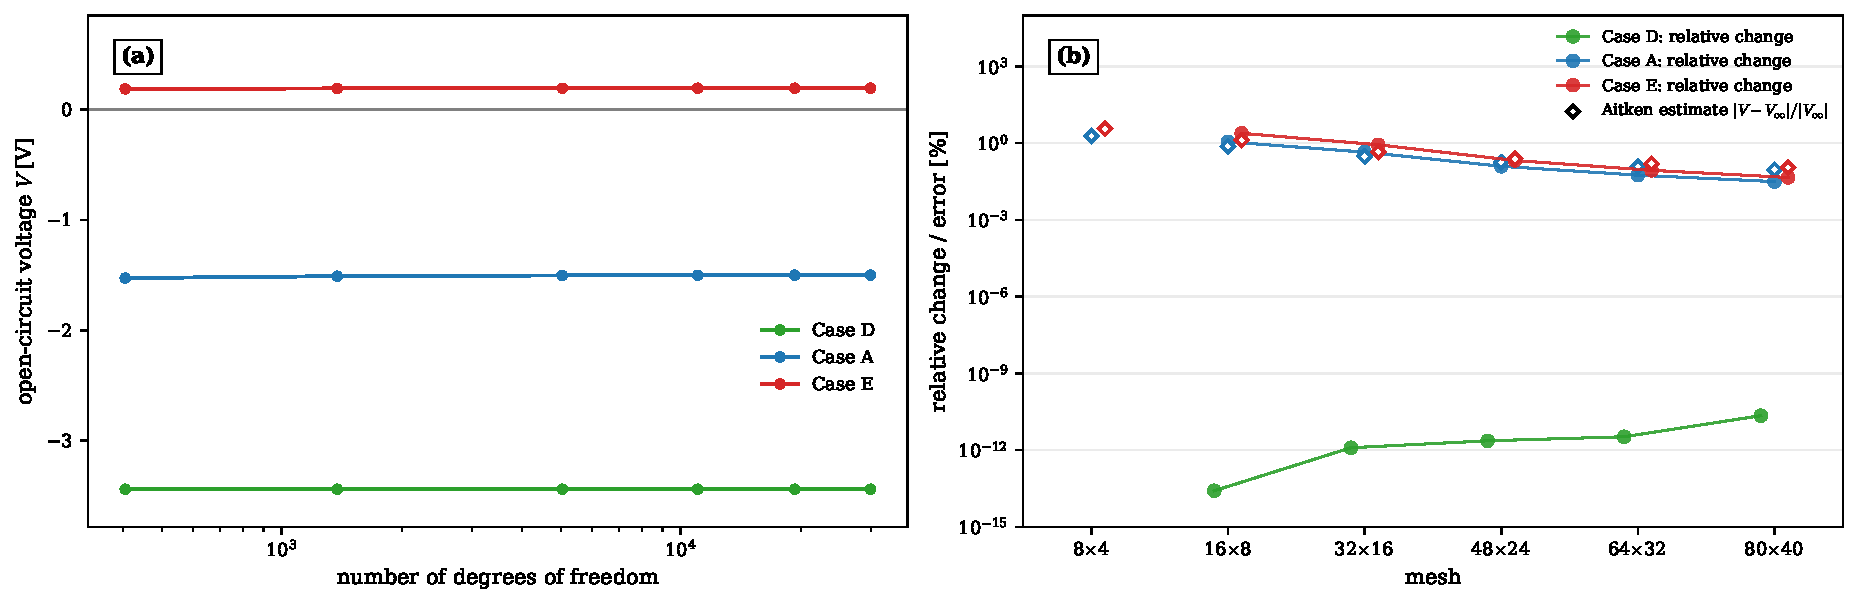
\includegraphics[width=\linewidth]{Fig2_mesh_convergence}
  \caption{Mesh convergence of Cases D, A and E over six refinement levels
  ($8\times4$ to $80\times40$). (a) Open-circuit voltage against the number of degrees
  of freedom. (b) Relative change from the previous level (circles) and
  extrapolation-based error estimate (diamonds), on a logarithmic scale.}
  \label{fig:fig02_mesh_convergence}
\end{figure}

Figure~\ref{fig:fig02_mesh_convergence} shows the same convergence study graphically.
In panel (a), the three voltages remain nearly unchanged over the refinement range.
Their relative positions and signs are also unchanged: Case~D is the most negative,
Case~A lies between Case~D and zero, and Case~E remains slightly positive. Even the
coarsest mesh places each voltage within about four per cent of its converged value.
Panel (b) shows the relative change on a logarithmic scale. For Cases~A and~E, the
relative change decreases from approximately one or two per cent at the second level
to a few hundredths of a per cent at the finest level. The corresponding trends are
consistent with the observed orders reported above. The extrapolation-based estimates
follow the same decreasing trend and remain close to the changes between successive
meshes. Case~D remains at the round-off level throughout, as expected because its
voltage does not depend on the mechanical solution. The smooth convergence of
Cases~A and~E is also consistent with the fact that the open-circuit voltage is an
integral quantity determined by the net charge on the electrode.

\subsection{Verification checks}
\label{sec:checks}

\begin{table}[t]
\centering
\small
\caption{Numerical verification: eleven checks of the discrete governing equations,
boundary conditions and algebraic structure of the discretization, together with two
reference values used elsewhere in the paper.}
\label{tab:verify}
\resizebox{\linewidth}{!}{%
\begin{tabular}{@{}llrl@{}}
\toprule
Check & Purpose & Residual & Tolerance \\
\midrule
BFS partition of unity & basis-function consistency & exact 0 & $<10^{-12}$ \\
BFS exact linear-field recovery & basis-function consistency & $2.1\times10^{-17}$ & $<10^{-12}$ \\
Coupled-block reciprocity, $K_{\phi u}=K_{u\phi}^{\!\top}$ & variational consistency & $1.3\times10^{-17}$ & $<10^{-12}$ \\
Case D vs.\ exact 1D pyroelectric result, $16\times8$ & analytical agreement & $1.3\times10^{-16}$ & $<10^{-10}$ \\
Case D vs.\ exact 1D pyroelectric result, $80\times40$ & analytical agreement & $1.5\times10^{-13}$ & $<10^{-10}$ \\
Zero-temperature null & null-limit consistency & exact 0 & $<10^{-12}$ \\
Zero-$\alpha$ null (Case E) & null-limit consistency & exact 0 & $<10^{-12}$ \\
Zero-$p$ null (Case D) & null-limit consistency & exact 0 & $<10^{-12}$ \\
Zero-$p$: Case A $\equiv$ Case E & null-limit consistency & exact 0 & $<10^{-10}$ \\
$p_3$-linearity at fixed $K$ (max.\ residual) & linearity of the algebraic system & $5.7\times10^{-15}$~V & $<10^{-9}$ \\
Stationary-potential/integrated-enthalpy identity & variational consistency & $3.5\times10^{-10}$ & $<10^{-7}$ \\
\midrule
Superposition defect $V_D+V_E-V_A$, $16\times8$ ($-1.7383$~V) & \multicolumn{3}{l}{reference value, Section~\ref{sec:voltages}} \\
Analytical 1D voltage ($-3.438647248$~V) & \multicolumn{3}{l}{reference value, Eq.~\eqref{eq:Vpyronum}} \\
\bottomrule
\end{tabular}%
}
\end{table}

Table~\ref{tab:verify} lists eleven verification checks, all satisfied within their
specified tolerances, together with two reference values used later. The first two
rows test the BFS basis by checking partition of unity and exact recovery of a linear
field. The reciprocity check verifies that the coupling blocks are transposes of one
another, as required by the single potential \eqref{eq:H}. The two Case~D checks
compare the finite-element solution with the closed-form result
\eqref{eq:Vpyronum} on a coarse and a fine mesh. The four null checks switch off the
temperature, thermal expansion, or pyroelectric coefficient and verify the corresponding
zero response or the reduction of Case~A to Case~E. The final two checks test the
linearity in $p_3$ and the stationary-potential identity. The latter involves
cancellation between terms of comparable magnitude and is therefore evaluated against
a less stringent tolerance than the other checks. Together, these tests verify the
discrete implementation of the governing equations and their coupling.

\paragraph{Energy balance}
At the solved state of Case~A ($80\times40$ mesh), the discrete electric enthalpy
splits into the five active terms of \eqref{eq:H} integrated over the domain,
\begin{align}
\Pi=\ &
\underbrace{4.6528\times10^{-8}}_{\mbox{\normalsize elastic, $\tfrac12\varepsilon^\top C\varepsilon$}}
\ \underbrace{-\,7.4376\times10^{-9}}_{\mbox{\normalsize $-\tfrac12E^\top\kappa E$}}
\ \underbrace{-\,1.9149\times10^{-8}}_{\mbox{\normalsize $-e\varepsilon\cdot E$}}
\notag\\
&\underbrace{-\,7.3907\times10^{-8}}_{\mbox{\normalsize $-\beta_{\mathrm{PS}}\theta\cdot\varepsilon$}}
\ \underbrace{+\,3.4024\times10^{-8}}_{\mbox{\normalsize $-p\theta\cdot E$}}
=-1.9941\times10^{-8}\ \text{J\,m}^{-1},
\label{eq:energyaudit}
\end{align}

The strain-gradient and flexoelectric terms are zero in all reported cases. The sum
agrees with an independent evaluation of the discrete potential,
$\tfrac12q^\top Kq-q^\top f=-1.99411\times10^{-8}\,\text{J\,m}^{-1}$, to a relative
error of $3.5\times10^{-10}$, consistent with the stationary-potential identity in
Table~\ref{tab:verify}. The individual terms show the relative contributions to the
discrete enthalpy. The thermal-stress work on the strain is the largest term in
magnitude and is balanced mainly by the elastic strain energy. The pyroelectric and
piezoelectric terms have opposite signs, consistent with the partial cancellation
between the two mechanisms discussed in Section~\ref{sec:voltages}. The dielectric
term is smaller than the other contributions.

\subsection{Linearity in the pyroelectric coefficient}
\label{sec:p3lin}

For Case~A on the $16\times8$ mesh, the open-circuit voltage was recomputed with $p_3$
multiplied by $0$, $0.5$, $1$, $1.5$ and $2$, with all other inputs, including the
stiffness matrix $K$, unchanged. Since $p_3$ enters only the load vector $f_\phi$,
the solution $q=K^{-1}f$ depends affinely on the scale factor. The computed voltages
follow a straight line to within $5.7\times10^{-15}$~V, with a slope of
$-1.7004$~V per unit scale factor.

\begin{figure}[t]
  \centering
  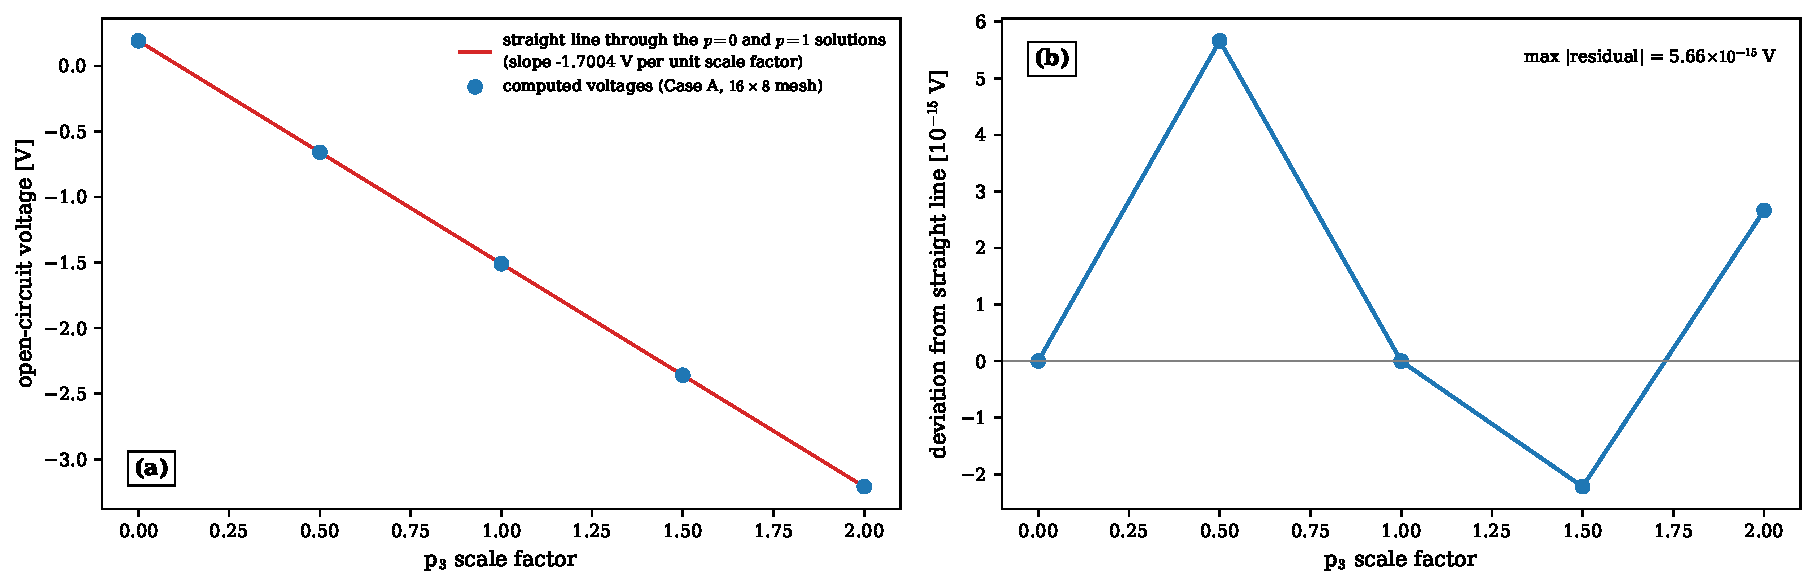
\includegraphics[width=\linewidth]{Fig3_p3_linearity}
  \caption{Dependence of the Case A voltage on the pyroelectric coefficient at fixed
  stiffness ($16\times8$ mesh). (a) Computed voltages against the $p_3$ scale factor,
  with the straight line through the $p=0$ and $p=1$ solutions. (b) Deviation from the
  straight line on an enlarged scale.}
  \label{fig:fig08_p3_sensitivity}
\end{figure}

Figure~\ref{fig:fig08_p3_sensitivity}(a) shows the computed voltage varying linearly
with the $p_3$ scale factor, from a small positive value at zero pyroelectric
coefficient to about $-3.2$~V at twice the nominal value. The value at zero scale
factor is the Case~E voltage on this mesh, because Case~A without the pyroelectric
term reduces to Case~E. The line therefore separates the Case~A voltage into an
intercept associated with the piezoelectric-thermal contribution and a term proportional
to $p_3$. At the nominal coefficient, the latter is $-1.70$~V, about half of the
Case~D voltage of $-3.44$~V obtained without piezoelectric coupling. In Case~A, the
pyroelectric field also contributes to the converse piezoelectric response; the
resulting deformation generates an additional piezoelectric charge that partially
opposes the direct pyroelectric contribution. Panel~(b) shows deviations from the
straight line on an enlarged scale. They are of order $10^{-15}$~V and change sign
irregularly between points, consistent with round-off rather than a physical
nonlinearity. Parameters that enter $K$ itself, such as an active flexoelectric
coupling, would not preserve this same affine dependence.


%======================================================================
\section{Results and Discussion}
\label{sec:results}
%======================================================================

\subsection{Open-circuit voltages of the three cases}
\label{sec:voltages}

\begin{table}[t]
\centering
\caption{Open-circuit voltages on the $80\times40$ mesh (29{,}889 degrees of freedom)
with the estimated discretization uncertainty.}
\label{tab:results}
\begin{tabular}{@{}llrl@{}}
\toprule
Case & Active mechanisms & $V$ (V) & Uncertainty \\
\midrule
D & pyroelectric only & $-3.43865$ & exact 1D result \\
A & piezoelectric + pyroelectric & $-1.49960$ & $\pm0.09\%$ \\
E & piezoelectric + thermal (no pyroelectric) & $+0.19321$ & $\pm0.15\%$ \\
\bottomrule
\end{tabular}
\end{table}

Table~\ref{tab:results} gives the open-circuit voltages for the three cases. The
pyroelectric response alone (Case~D) produces $-3.43865$~V, with the sign determined
by the negative primary pyroelectric coefficient. The piezoelectric-thermal response
alone (Case~E) is $+0.19321$~V, about eighteen times smaller in magnitude and of
opposite sign. When both mechanisms are active (Case~A), the voltage is
$-1.49960$~V. The difference between Cases~D and~E reflects the different coupling
paths. In Case~D, the temperature directly enters the electric displacement through
the pyroelectric term. In Case~E, the temperature first produces a strain field
through thermal expansion and mechanical compatibility, which then contributes to the
electric response through the piezoelectric coupling. The two mechanisms therefore
do not combine by simply adding the separately computed Case~D and Case~E voltages:
$V_D+V_E\approx-3.25$~V, whereas the coupled Case~A voltage is much less negative.
As shown in Section~\ref{sec:p3lin}, piezoelectric coupling also modifies the
pyroelectric contribution itself. Thus, the two mechanisms partially oppose one
another in the coupled response.

\begin{figure}[t]
  \centering
  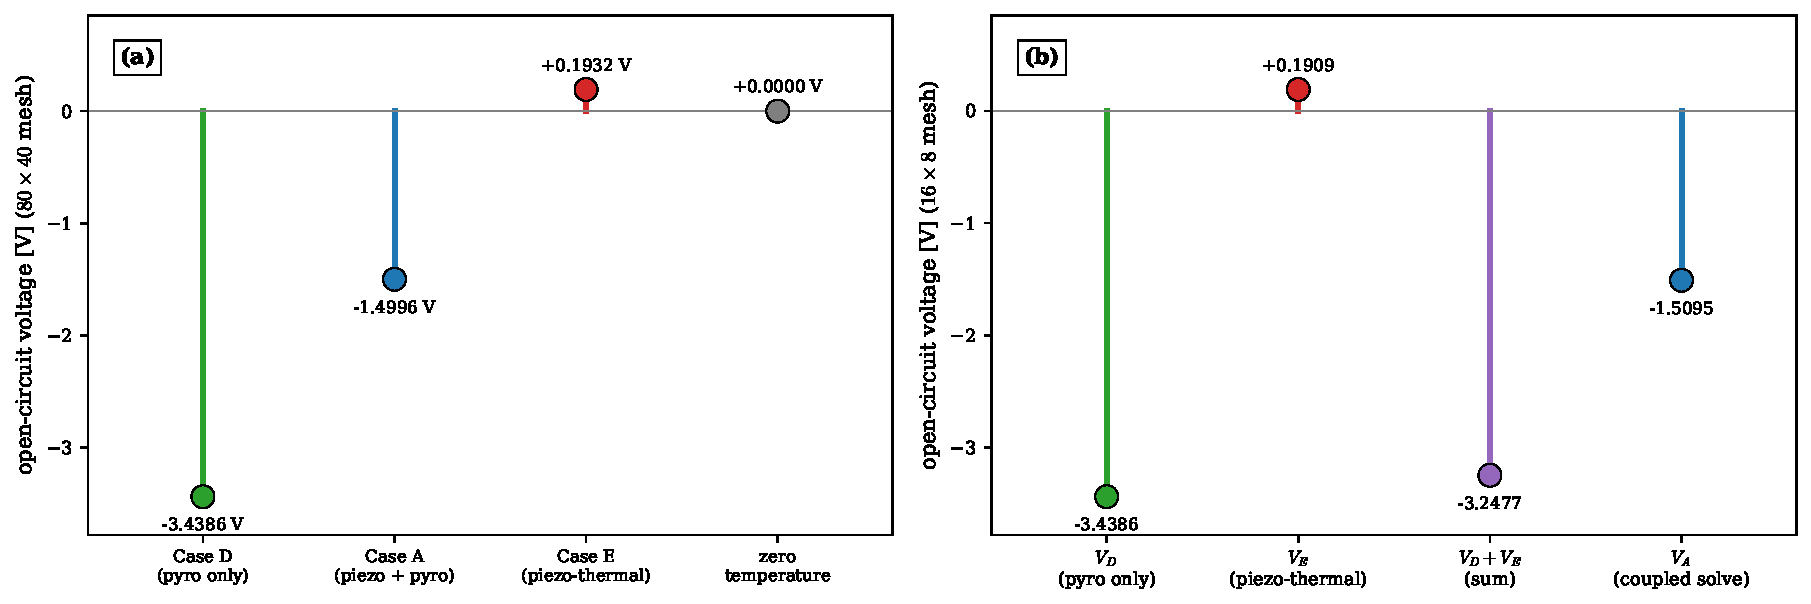
\includegraphics[width=\linewidth]{Fig4_voltages_decomposition}
  \caption{Open-circuit voltages and their decomposition. (a) Converged voltages of
  Cases D, A and E ($80\times40$ mesh) and of the zero-temperature case. (b) Comparison
  on a common $16\times8$ mesh showing $V_D+V_E\neq V_A$.}
  \label{fig:fig03_cases_and_decomposition}
\end{figure}

Figure~\ref{fig:fig03_cases_and_decomposition}(a) presents the converged voltages as
stems from zero. The pyroelectric-only stem is the longest and points downward, the
combined stem also points downward but reaches less than half as far, and the
piezoelectric-thermal stem is short and points upward. The zero-temperature case
remains exactly at zero. This confirms that the reported voltages arise from the
prescribed temperature field rather than from a residual numerical offset. Panel~(b)
repeats the comparison on a common $16\times8$ mesh and includes the sum $V_D+V_E$.
This sum is about $-3.25$~V, whereas the solved Case~A voltage is about $-1.51$~V.
The difference, about 1.74~V, is much larger than the magnitude of the
piezoelectric-thermal voltage alone. The reason is that Case~D is obtained without
piezoelectric coupling, whereas in Case~A the pyroelectric field also produces a
converse piezoelectric deformation and the associated piezoelectric charge. Because
the system is linear in the thermal load, the coupled Case~A response can instead be
viewed as the Case~E contribution plus a pyroelectric contribution evaluated with the
piezoelectric coupling active. A separate one-dimensional pyroelectric estimate
combined with an independently computed piezoelectric-thermal correction would
therefore not reproduce the coupled device voltage.

\subsection{Solved fields}
\label{sec:fields}

\begin{figure}[t]
  \centering
  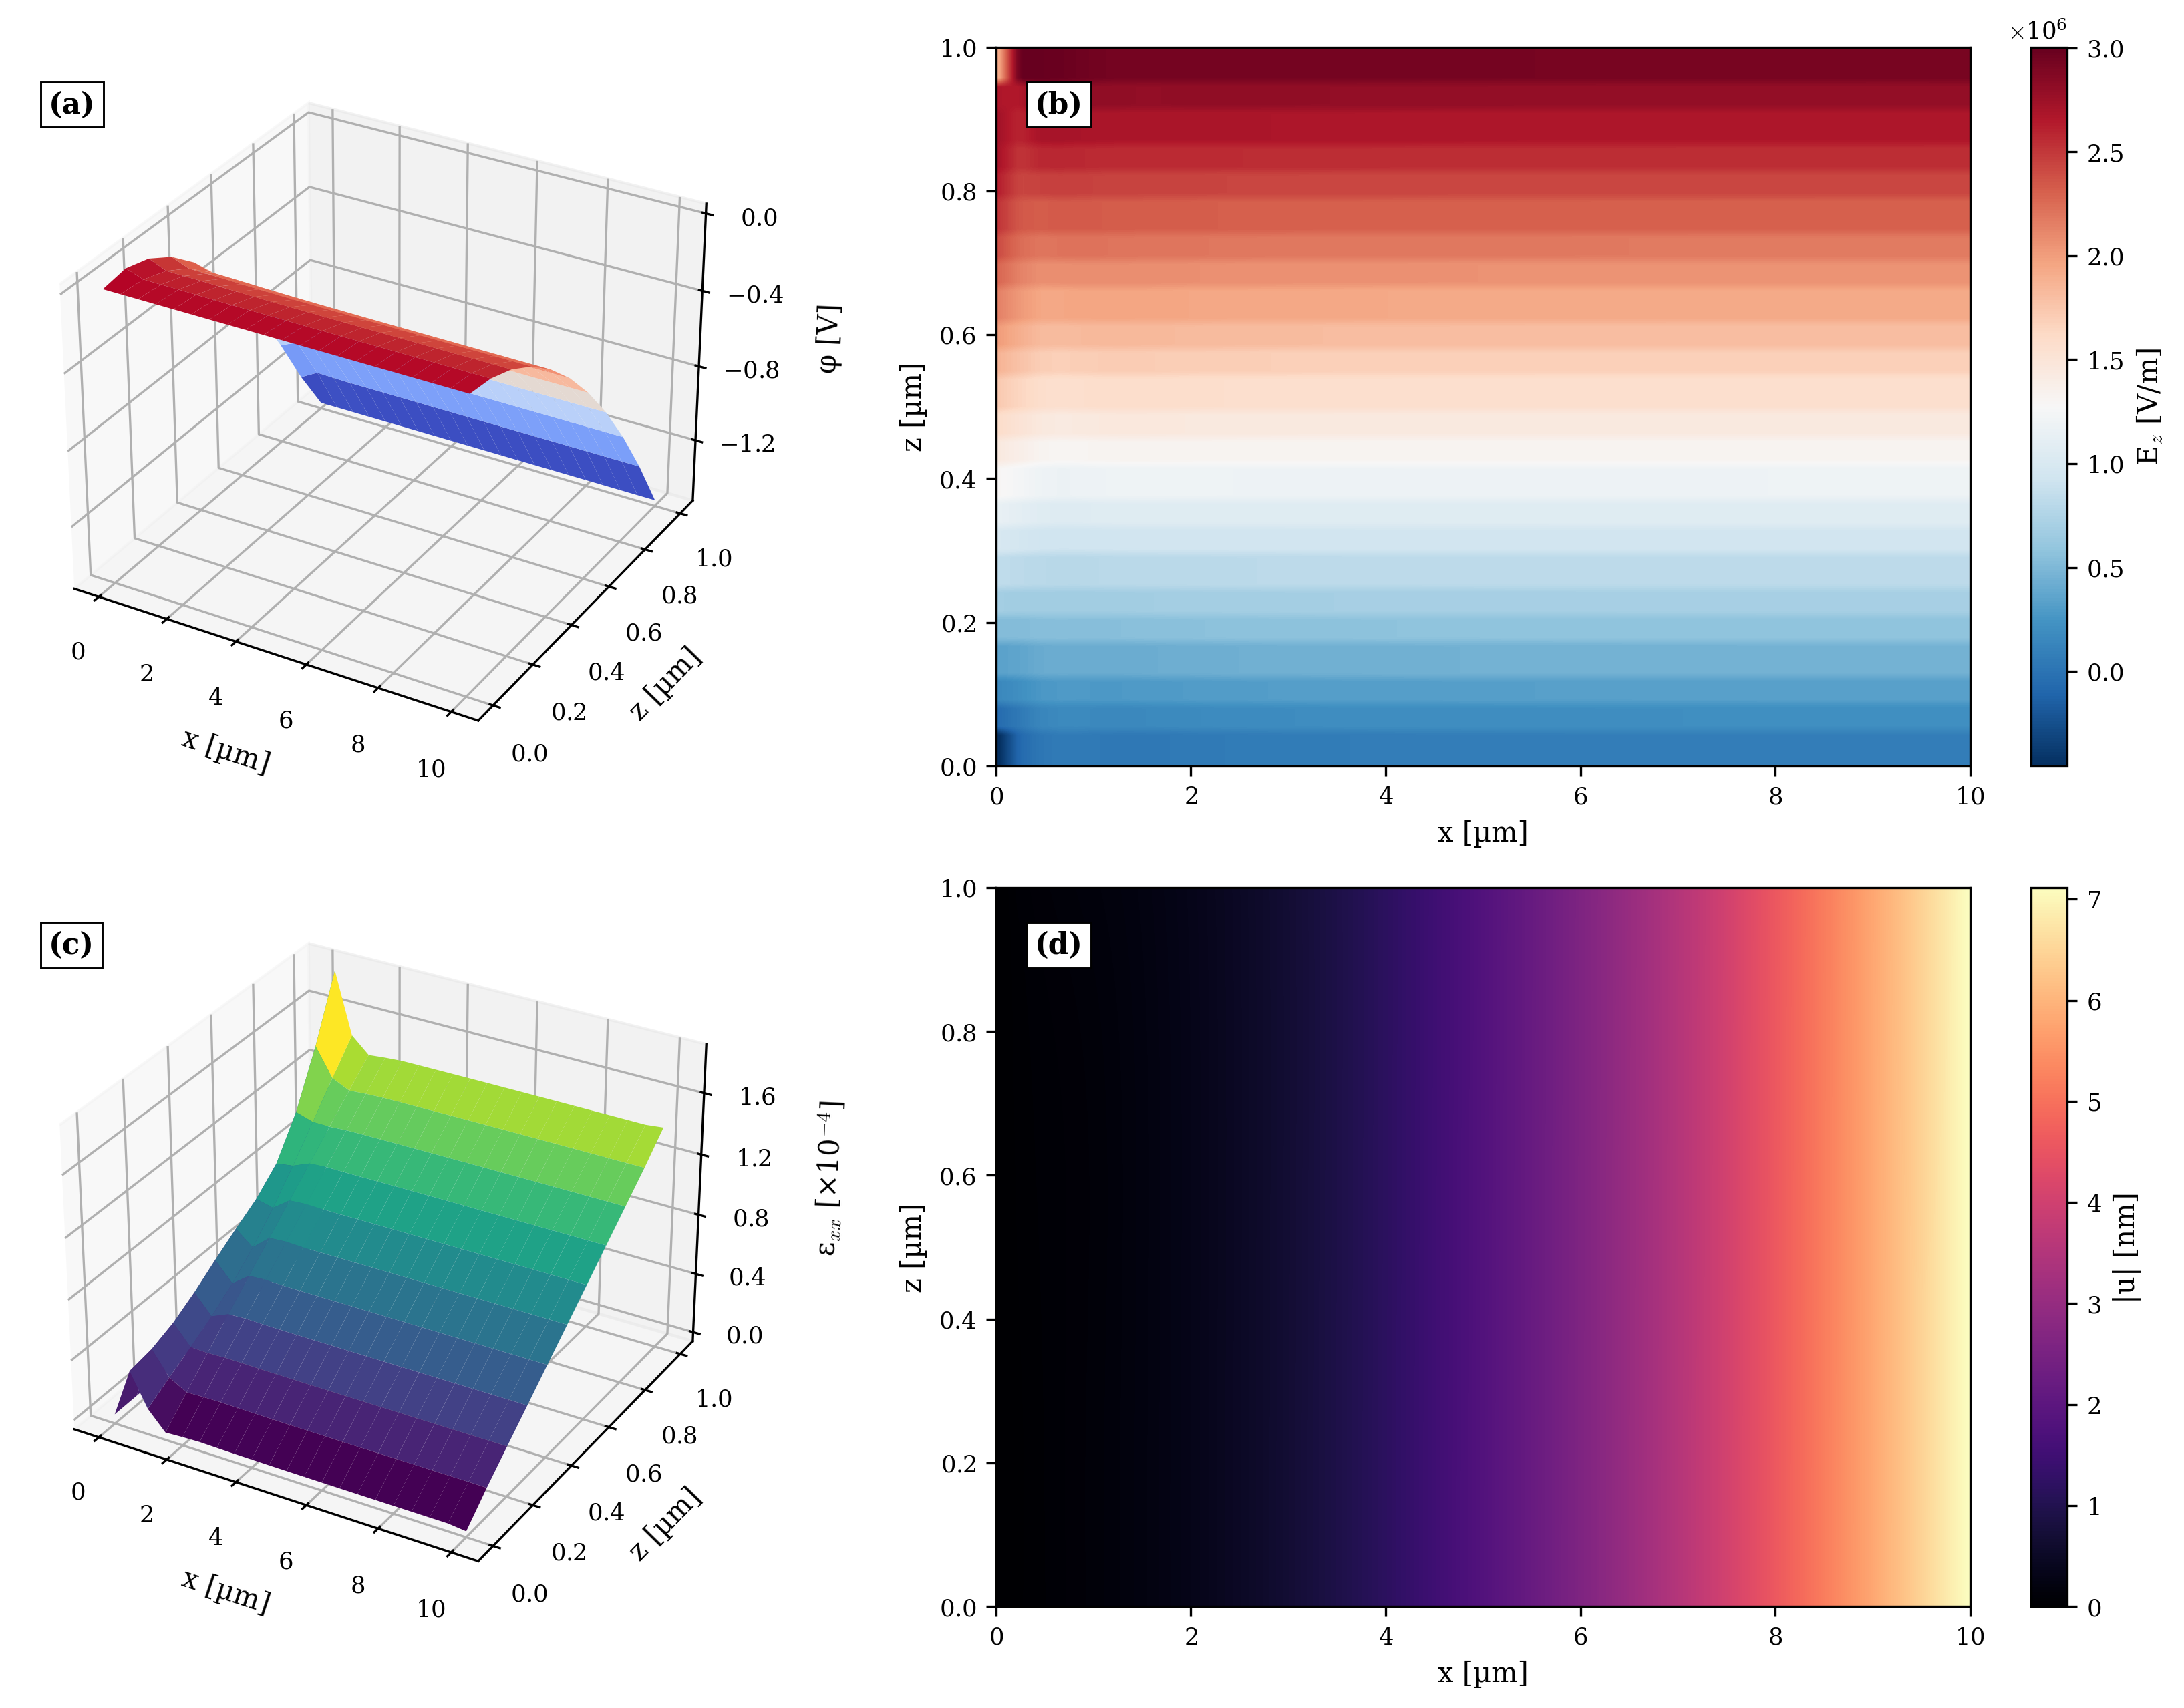
\includegraphics[width=\linewidth]{Fig5_solved_fields.png}
  \caption{Solved fields of Case A ($48\times24$ mesh), evaluated from the
  finite-element basis at physical points. (a) Electric potential. (b) Through-thickness
  electric field $E_z$. (c) Longitudinal strain $\varepsilon_{xx}$. (d) Displacement
  magnitude $|\mathbf{u}|$.}
  \label{fig:fig04_solved_fields}
\end{figure}

Figure~\ref{fig:fig04_solved_fields} shows the solved fields for Case~A over the
specimen. In panel (a), the potential is zero on the grounded bottom face and reaches
about $-1.5$~V on the top face. Along the span, the top surface is nearly at a single
potential, apart from a small disturbance near the clamped root, consistent with the
floating equipotential electrode condition. Through the thickness, the potential is
nonlinear: its variation is smaller near the bottom and larger near the top. Panel
(b) shows the corresponding $E_z$ field. The field forms approximately horizontal
bands, increasing from nearly zero at the cool bottom face to about
$3\times10^{6}$~V\,m$^{-1}$ near the hot top face, with little variation along the
span. This follows the linear temperature dependence of the pyroelectric charge
density $p_3\theta$. The top-field magnitude is somewhat less than half of the value
$-p_3\theta/\kappa_{33}$ obtained from the pyroelectric-only response, consistent with
the reduction identified in Section~\ref{sec:p3lin}. Panel (c) shows the longitudinal
strain. Away from the root, $\varepsilon_{xx}$ varies approximately linearly from
nearly zero at the bottom to about $1.4\times10^{-4}$ at the top and is nearly uniform
along the span. The hotter upper region therefore undergoes greater longitudinal
strain than the cooler lower region. Near the clamped root, the strain develops a
sharp peak at the top corner, corresponding to the Saint-Venant boundary layer, which
decays within approximately one thickness. Panel (d) shows the displacement
magnitude, increasing from zero at the clamp to about 7~nm at the free end and
remaining nearly uniform through the thickness. The beam therefore undergoes overall
bending under the imposed temperature difference. The four fields together show that
the electrical response follows the through-thickness temperature variation, while
the mechanical response produces a non-uniform strain field that contributes to the
piezoelectric charge.

\subsection{Origin of the non-uniform strain}
\label{sec:clamp}

The clamp at $x=0$ is the only external mechanical constraint in the model, so it is
useful to examine whether it controls the non-uniform strain responsible for Case~E.
To this end, Case~E was solved for spans
$L\in\{10,20,50,100,200,500\}\,\mu\text{m}$ with the thickness, thermal load, and
production element length (0.125~$\mu$m along $x$) kept fixed. The voltage increases
from $+0.1932$~V at $L=10\,\mu\text{m}$ to $+0.1975$~V for the longest span, an
increase of about 2\%. It is already within about 1\% of this long-span value at
$L=20\,\mu\text{m}$. The remaining difference decreases approximately in proportion
to $1/L$, consistent with a correction confined to a region of fixed size near the
ends. Thus, as the span increases, the contribution associated with the root region
becomes a smaller fraction of the specimen. The non-uniform strain instead persists
because of the temperature gradient itself. Each layer would undergo a different
thermal strain if unconstrained, since its temperature differs from that of adjacent
layers. Compatibility between the layers, together with the plane-strain condition
$\varepsilon_{yy}=0$, produces a strain field that varies through the thickness even
away from the clamp. Away from the root, the accompanying stresses are small: in a
$200\,\mu$m specimen, the midspan values of $\sigma_{xx}$ and $\sigma_{zz}$ are about
three orders of magnitude smaller than the thermal stress
$\beta_{\mathrm{PS}}\Delta T$ that the same temperature change would produce in a
fully constrained crystal, and they decrease further with mesh refinement. This is
consistent with the classical result that a linear temperature field leaves a free
beam or plate nearly stress-free ~\cite{BoleyWeiner1997}. Within the span range
examined here, the Case~E voltage is therefore controlled primarily by the
temperature-induced non-uniform strain rather than by the local root constraint.

\subsection{Effect of the thermal-stress reduction on polarity}
\label{sec:polarity}

On a common $48\times24$ mesh, the simplified thermal-stress vector of
Table~\ref{tab:beta} gives $V_A=-1.9093$~V and $V_E=-0.2154$~V, whereas the full
contraction \eqref{eq:betaPS} gives $V_A=-1.5009$~V and $V_E=+0.1930$~V; the
converged values are those of Table~\ref{tab:results}. Both voltages shift by the same
amount, $+0.408$~V, while Case~D, which does not involve $\beta_{\mathrm{PS}}$, is
unchanged. The equal shift follows from linearity: $\beta_{\mathrm{PS}}$ enters only
the mechanical load vector, so changing $\beta_{\mathrm{PS}}$ produces the same
mechanically generated voltage shift in the cases that contain piezoelectric coupling.
The terms omitted by the simplified reduction are positive in both components, so the
full contraction increases the thermal load and shifts the resulting
piezoelectric-thermal voltage toward the positive direction. In the present model,
the sign of the piezoelectric-thermal voltage is therefore particularly sensitive to
the thermal-stress reduction.

The sign cannot be inferred from the individual material coefficients alone. The
vector $\beta_{\mathrm{PS}}$ combines the positive $a$-axis coefficient and the
negative $c$-axis coefficient, weighted by elastic constants of similar magnitude
(Eq.~\eqref{eq:betaPS}). The resulting strain is then coupled through the
piezoelectric constants $e_{31}$ and $e_{33}$, which also have opposite signs. The
net voltage consequently results from the difference between several contributions,
and the full three-dimensional thermal contraction is required to determine it in the
present plane-strain formulation. The vector $\beta_{\mathrm{PS}}$ itself retains the
same sign under the two reductions (Table~\ref{tab:beta}); it is the voltage generated
through the resulting non-uniform strain of Section~\ref{sec:clamp} that changes sign.
For the combined device response, $|V_D|$ is much larger than $|V_E|$, so $V_A$
remains negative under both reductions, while the simplified reduction makes its
magnitude about 27\% too large. The sign reversal therefore occurs specifically in
the piezoelectric-thermal contribution.

\subsection{Sensitivity to the thermal-expansion coefficients}
\label{sec:alpha}

Because $V_E$ depends on $\beta_{\mathrm{PS}}$, and $\beta_{\mathrm{PS}}$ depends on
the fitted $\alpha_1$ and $\alpha_3$ (Section~\ref{sec:materials}), the sensitivity
of the voltage to the fitting uncertainty was examined. The two coefficients are
fitted separately to the $a(T)$ and $c(T)$ data and are treated as independent.
Perturbations are propagated as
\begin{equation}
V_E(\alpha_1+\delta_1,\alpha_3+\delta_3)\approx
V_E(\alpha_1,\alpha_3)
+\frac{\partial V_E}{\partial\alpha_1}\delta_1
+\frac{\partial V_E}{\partial\alpha_3}\delta_3,
\qquad
\delta_i=n_i\,\mathrm{SE}(\alpha_i),
\label{eq:uncertaintyprop}
\end{equation}
with $\mathrm{SE}(\alpha_1)=1.6459\times10^{-6}\,\text{K}^{-1}$ and
$\mathrm{SE}(\alpha_3)=3.2611\times10^{-6}\,\text{K}^{-1}$, by direct re-solution of
the $80\times40$ model at the perturbed values. Over one standard deviation in both
coefficients ($n_i=\pm1$), $V_E$ remains between $+0.062$ and $+0.324$~V, so its
positive polarity is preserved. Over two standard deviations, $V_A$ remains between
$-1.762$ and $-1.237$~V and does not change sign. The voltage is more sensitive to
$\alpha_3$ than to $\alpha_1$: one standard deviation of $\alpha_3$ changes $V_E$ by
about 0.11~V, compared with about 0.025~V for $\alpha_1$. The Case~E voltage becomes
negative only when $\alpha_3$ is taken close to two standard deviations more negative
than the fitted value.

To examine the dependence over a wider range, the model was also solved on a $3\times3$
grid in which $\alpha_1$ and $\alpha_3$ are each scaled by 0.5, 1 and 1.5
($48\times24$ mesh). This grid extends well beyond the uncertainty band; for example,
its lowest value of $\alpha_1$ lies about 6.6 standard deviations below the fitted
value. Figures~\ref{fig:fig05_alpha_grid_3d}--\ref{fig:fig07_sign_evidence} show the
nine solved points directly, without interpolation.

\begin{figure}[t]
  \centering
  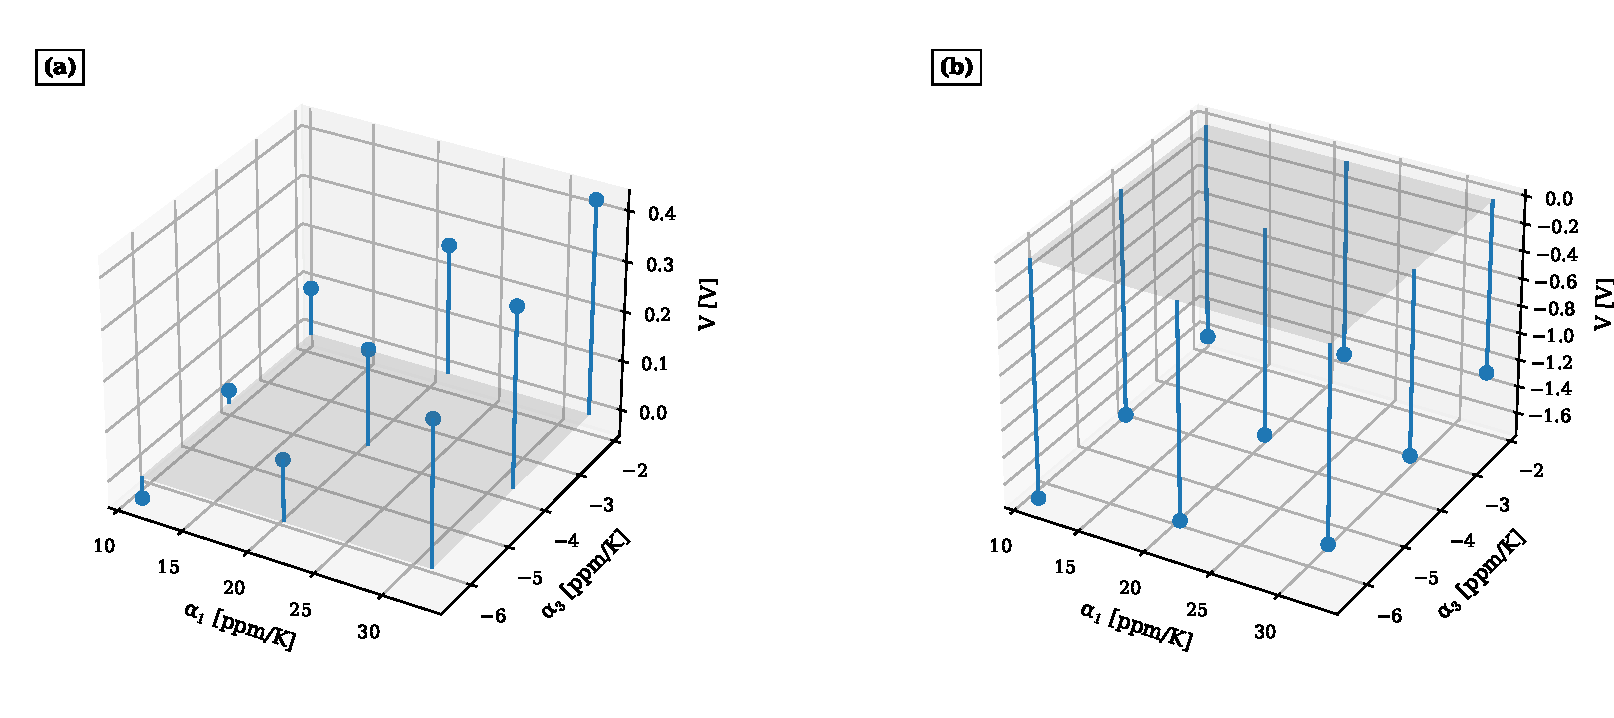
\includegraphics[width=\linewidth]{Fig6_alpha_grid_3d}
  \caption{Voltages on the $3\times3$ grid of scaled thermal-expansion coefficients,
  shown as stems over the $(\alpha_1,\alpha_3)$ plane with a zero-reference plane.
  (a) Case E. (b) Case A.}
  \label{fig:fig05_alpha_grid_3d}
\end{figure}

Figure~\ref{fig:fig05_alpha_grid_3d}(a) shows the Case~E voltage as stems over the
$(\alpha_1,\alpha_3)$ plane. The stems increase in height as $\alpha_1$ increases
and decrease as $\alpha_3$ becomes more negative. Eight of the nine stems point
upward; the single downward stem lies just below zero at the combination of the
smallest $\alpha_1$ and most negative $\alpha_3$. The stem tips lie on a tilted plane,
because the voltage is linear in both coefficients: $\beta_{\mathrm{PS}}$ is linear in
$\alpha$, and the coupled system is linear in $\beta_{\mathrm{PS}}$. The two
coefficients therefore contribute with opposite tendencies: increasing the in-plane
expansion increases the positive piezoelectric-thermal voltage, whereas a stronger
contraction along the $c$ axis acts in the opposite direction. Panel (b) shows the
same grid for Case~A. All stems point downward, between about $-1.74$ and $-1.26$~V,
and their tips form a plane with the same tilt as in panel (a). The combined voltage
becomes less negative as $\alpha_1$ increases because the opposing
piezoelectric-thermal contribution increases. The pyroelectric contribution therefore
remains the dominant contribution to the sign of the combined voltage over this grid.

\begin{figure}[t]
  \centering
  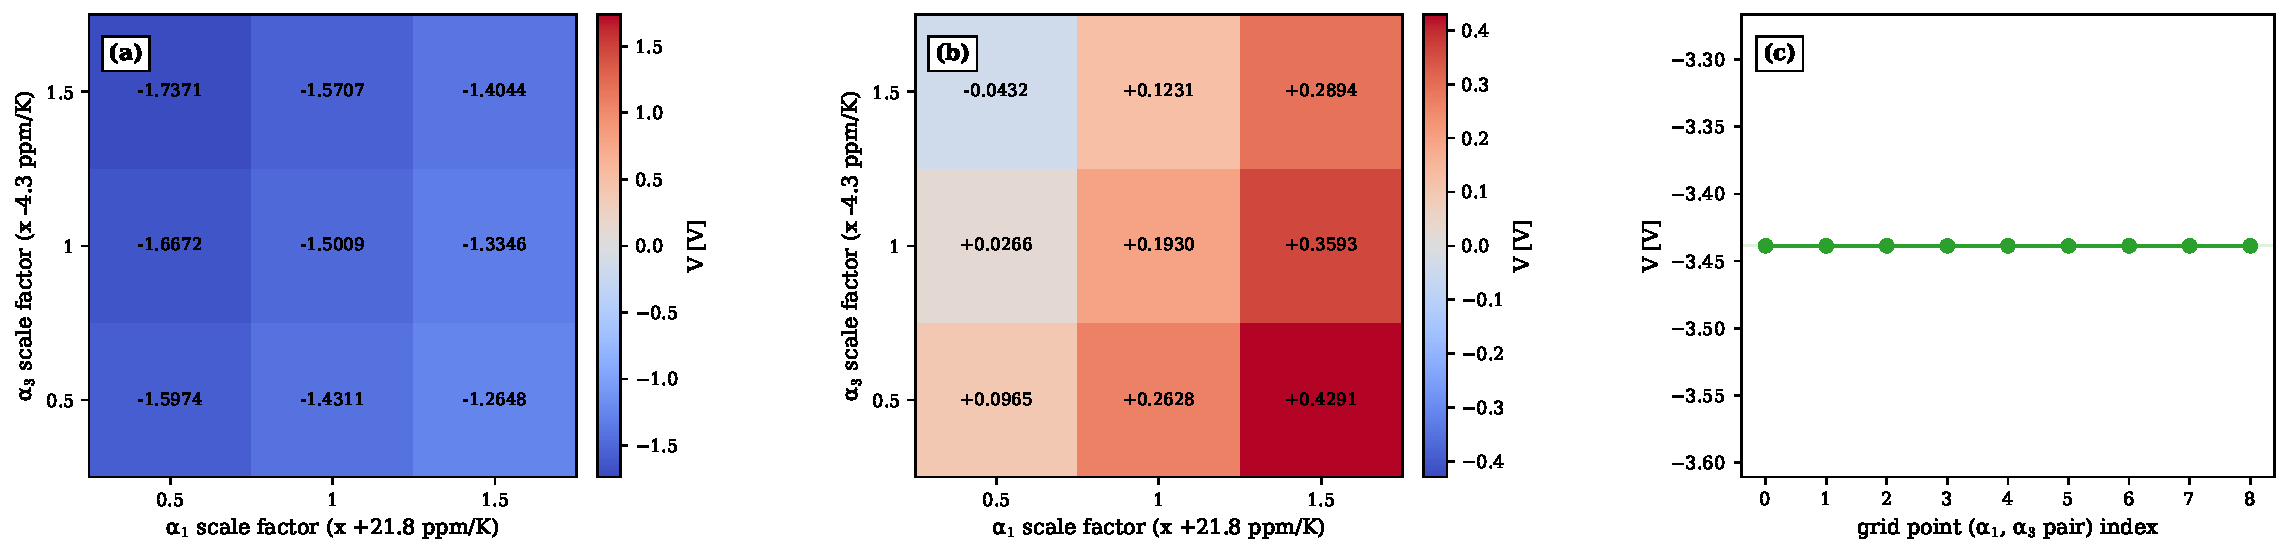
\includegraphics[width=\linewidth]{Fig7_alpha_grid_maps}
  \caption{The same $3\times3$ grid as annotated maps. (a) Case A. (b) Case E. (c)
  Case D for all nine coefficient pairs.}
  \label{fig:fig06_alpha_grid_heatmap}
\end{figure}

Figure~\ref{fig:fig06_alpha_grid_heatmap} gives the same results as annotated maps,
which make the regular dependence easier to inspect. In panels (a) and (b), the
voltage changes in equal increments across each row and column: each half-step in
the scale of $\alpha_1$ changes the voltage by the same amount, and the same applies
to each half-step in the scale of $\alpha_3$. Per unit change of the coefficient, the
voltage is about twice as sensitive to $\alpha_3$ as to $\alpha_1$, consistent with
the larger contribution of $\alpha_3$ to the uncertainty of the result. A
cell-by-cell comparison of the two maps shows that $V_A-V_E$ has the same value,
about $-1.69$~V, in all nine cells. Thus, over this coefficient grid, the
pyroelectric contribution to Case~A is independent of the thermal-expansion
coefficients, and the variation of the combined voltage with $\alpha$ enters through
the piezoelectric-thermal contribution. The Case~E map is positive everywhere except
in the one corner cell, where the value is close to zero. Panel (c) shows Case~D at
all nine points as a flat line at the analytical value. The pyroelectric-only voltage
is independent of the thermal expansion, confirming that thermal expansion affects
the voltage through the piezoelectric route.

\begin{figure}[t]
  \centering
  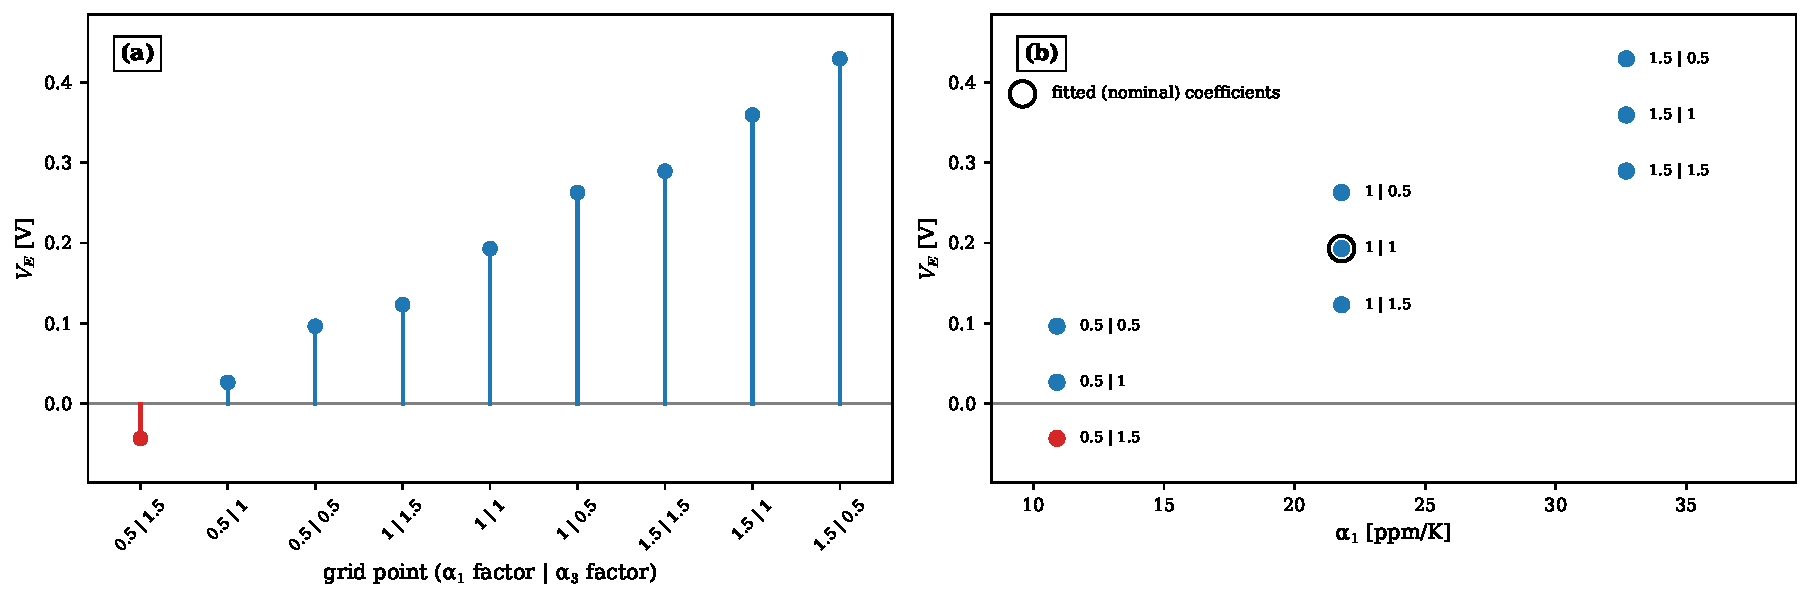
\includegraphics[width=\linewidth]{Fig8_sign_of_caseE}
  \caption{Sign of the Case E voltage over the $3\times3$ grid. (a) The nine values in
  increasing order, labelled by their $\alpha_1$ and $\alpha_3$ scale factors. (b) The
  same values against $\alpha_1$, with the fitted (nominal) pair marked.}
  \label{fig:fig07_sign_evidence}
\end{figure}

Figure~\ref{fig:fig07_sign_evidence} focuses on the sign of the Case~E voltage. Panel
(a) arranges the nine values in increasing order. Eight are positive, ranging from
just above zero to about $+0.43$~V. The single negative value is small and close to
zero and occurs for the pair with halved $\alpha_1$ and enlarged $|\alpha_3|$.
Panel (b) plots the same values against $\alpha_1$. The points form three vertical
columns, one for each value of $\alpha_1$, while the spread within each column is
caused by $\alpha_3$. The columns move upward as $\alpha_1$ increases, and the
nominal point lies in the middle column, well above zero. The negative value belongs
to the lowest $\alpha_1$ level and the most negative $\alpha_3$, which is also the
corner of the grid farthest from the fitted coefficients. Within the tested parameter
grid, the sign of the piezoelectric-thermal voltage is therefore sensitive to the
thermal anisotropy of tetragonal BaTiO$_3$. The same dependence indicates that
thermal-expansion anisotropy provides a parameter through which the magnitude and
sign of the piezoelectric-thermal contribution can be shifted.

\subsection{Comparison with a one-dimensional estimate}
\label{sec:estimate}

A simple estimate of the piezoelectric-thermal voltage replaces $p_3$ in
\eqref{eq:Vpyro} by the free-sample secondary combination
$2e_{31}\alpha_1+e_{33}\alpha_3$
($-59\,\mu\text{C\,m}^{-2}\text{K}^{-1}$, Section~\ref{sec:materials}):
\begin{equation}
V_{\mathrm{piezo\text{-}th}}^{\mathrm{1D}}
\approx
\frac{(2e_{31}\alpha_1+e_{33}\alpha_3)\bar\theta h}{\kappa_{33}}
=
\frac{(-5.933\times10^{-5})(5)(1.0\times10^{-6})}
{4.95834517752\times10^{-10}}
=-0.598\,\text{V},
\label{eq:Vpt}
\end{equation}
Since this is a free-sample estimate, the free permittivity
$\varepsilon_{33}^T=132.4\,\varepsilon_0$ may be used instead of the clamped value,
which gives $-0.253$~V. Both estimates have the sign opposite to the finite-element
result of $+0.193$~V. The estimate assumes that each material point undergoes its
free thermal strain independently of its neighbours. In the cantilever, the
through-thickness temperature variation and compatibility between neighbouring
layers produce a non-uniform strain field (Section~\ref{sec:clamp}), and the strain
entering the piezoelectric constitutive relation therefore differs from the free
thermal strain in both magnitude and spatial distribution. Within the terminology
used for pyroelectric effects, Case~E can therefore be viewed as a
finite-element realization of the tertiary pyroelectric effect
~\cite{Lang2005Pyro} for this specimen and support, distinct from the primary
mechanism represented by Case~D and from the free-sample secondary estimate in
\eqref{eq:Vpt}. The comparison shows that the piezoelectric-thermal voltage of this
temperature-gradient device cannot be obtained from the free-sample secondary
coefficient alone; the coupled strain field is required to determine both its
magnitude and, in this case, its sign.

%======================================================================
\section{Conclusions}
\label{sec:conclusions}
%======================================================================

This paper developed a coupled finite-element model, based on a single electric
enthalpy and a $C^1$ Bogner--Fox--Schmit element, for the open-circuit voltage of a
plane-strain tetragonal BaTiO$_3$ microcantilever under a through-thickness temperature
difference. The model treats the pyroelectric and piezoelectric-thermal mechanisms
together, forms the plane-strain thermal stress from the full three-dimensional
contraction, and uses the fixed-strain pyroelectric coefficient. The main findings are
as follows.

\begin{itemize}
\item The plane-strain thermal-stress vector of a tetragonal crystal must be formed
from the full three-dimensional contraction before the plane-strain condition is
applied. The simplified reduction omits the contribution associated with the blocked
out-of-plane expansion and underestimates the axial and through-thickness thermal
stresses by about 35\% and 58\%, respectively.

\item This difference reverses the sign of the piezoelectric-thermal voltage, from
$-0.22$~V with the simplified reduction to $+0.19$~V with the full contraction, and
makes the combined voltage about 27\% too large in magnitude. The same thermal-stress
change produces the same voltage shift in the coupled cases because the system is
linear in the thermal load.

\item The pyroelectric-only voltage, $-3.44$~V, agrees with the exact one-dimensional
result to round-off. Using the fixed-strain coefficient rather than the total
coefficient gives a magnitude about 27\% larger for the pyroelectric-only voltage and
avoids including the strain-mediated secondary contribution separately through the
material coefficient in the coupled formulation.

\item When both mechanisms act, the voltage is $-1.50$~V. The piezoelectric-thermal
part opposes the pyroelectric part, while the piezoelectric coupling also modifies the
pyroelectric contribution itself. The combined voltage is therefore not obtained by
simply adding the separately computed Case~D and Case~E voltages.

\item The piezoelectric-thermal voltage is produced primarily by the non-uniform strain
associated with the temperature gradient under plane strain rather than by the local
root constraint. It changes by only about 2\% when the span is increased from
$10$ to $500\,\mu\text{m}$. Within the terminology used for pyroelectric effects, this
response corresponds to a tertiary pyroelectric contribution for the present specimen
and support, and it cannot be obtained from the free-sample secondary coefficient
alone.

\item The positive polarity of the piezoelectric-thermal voltage is preserved over one
standard deviation of the fitted thermal-expansion coefficients. Over the wider parameter grid examined, the piezoelectric-thermal voltage depends
linearly on both thermal-expansion coefficients, with the $c$-axis coefficient
producing the larger change per unit variation.
\end{itemize}

The present results are relevant to a broader class of thermo-electro-mechanical
microdevices in which a temperature gradient is converted into an electrical signal.
Directly, the model is relevant to pyroelectric infrared detectors, thermal-imaging
pixels, temperature sensors, and microscale thermal sensing elements based on
ferroelectric or piezoelectric materials. The predicted piezoelectric-thermal
contribution is also relevant to devices in which thermal gradients generate mechanical
strain and, consequently, an additional electrical response, including thermally
responsive microcantilevers, resonant microsystems, and pyroelectric--piezoelectric
energy-conversion elements. More generally, the results are useful for the
interpretation and design of coupled thermo-electro-mechanical components in
microelectromechanical systems (MEMS), where geometric constraint and anisotropic
thermal expansion can affect not only the magnitude but also the polarity of the
electrical output. The present calculations therefore provide a modelling framework
for assessing these effects before experimental device-level characterization.


\subsection*{Scope and limitations}
The polarity predictions apply to the stated linear constitutive model,
plane-strain kinematics, prescribed steady temperature field and ideal electrode
conditions. They should not be interpreted as geometry-independent material
properties. The exact pyroelectric limit and discrete consistency checks verify
parts of the implementation, but do not replace independent validation of the full
coupled boundary-value problem. A three-dimensional or plane-stress comparison and
experimental device-level characterization remain outside the present study.
The calculations do not establish sensor sensitivity, harvested power or conversion
efficiency. Although a higher-order extension is described, the reported voltages
exclude flexoelectricity and do not establish a flexoelectric size effect.

\backmatter
\bmhead{Acknowledgements}
Vipin Gupta gratefully acknowledges the financial support provided by the Haryana
State Higher Education Council (HSHEC), Government of Haryana, through the Haryana
State Research Fund (HSRF) scheme (Sanction Letter
No.~14/66-2026 SPD/HSHEC/HSRF-38).

\section*{Declarations}
\bmhead{Funding}
Support from HSHEC through the HSRF scheme is acknowledged above.
\bmhead{Competing interests}
No potential conflict of interest was reported by the authors.
\bmhead{Data availability}
Data supporting the findings are available from the corresponding author upon
reasonable request.
% Author contributions must be supplied/confirmed by all authors before submission.

\bibliography{references}
\end{document}
